%03introduction.tex

\chapter{Management summary}
\section{Ausgangslage}
Je nach Untergrund, Bodeneigenschaften, Gel\"ande sowie Klima gedeihen in der Schweiz unterschiedliche Typen von W\"aldern. Seit einigen Jahrzehnten werden diese Typen von Experten erhoben und kartiert. Es wurden dabei verschiedene typisierte Waldstandorte festgelegt. Aktuell werden Karten, die im Auftrag der Kantone von Experten angefertigt wurden, nur in grossen Intervallen revidiert, wobei sie oft auch nicht fl\"achendeckend vorhanden sind (z.B. in den Kantonen GR, VS, BE).
Einer der Gr\"unde daf\"ur sind u.a. die hohen Kosten, die eine Analyse im Feld mit sich bringt.
Zudem ist die Erfassung und Nachf\"uhrung der Karten gepr\"agt von analogen Vorg\"angen, da die vorhandenen
technischen Ger\"ate und Programme f\"ur den Einsatz im Feld ungeeignet sind.
Daher muss von Hand Niedergeschriebenes im B\"uro oder von staatlichen Institutionen digitalisiert werden, bevor es an den
Arbeitgeber geschickt werden und sp\"ater auf kantonal isolierten Plattformen publiziert werden kann.

\section{Ziel der Arbeit}
Die Erfassung und Publikation von Waldstandorten sollte vereinfacht und beschleunigt werden. Dabei
sollen digitale Technologien eingesetzt werden wie Smartphone, GPS und Internet. Diese neuen
Instrumente sollen entsprechend geschulten Nutzern die Erfassung von Waldstandorten erm\"oglichen sowie \"offentliche und private Informationen in Form von Fl\"achen und Punkten. Auf einer Basis - Karte wird mittels GPS die eigene
Position angezeigt. Dar\"uber werden umliegende, bereits erfasste Waldstandorte, \"offentliche Fl\"achen anderer sowie die eigenen, privaten Fl\"achen dargestellt. Diese Fl\"achen k\"onnen Waldstandorte beschreiben oder aber zus\"atzliche Informationen \"uber den Standort beinhalten, z.B. eine speziell gekennzeichnete Beobachtungsfl\"ache.

\section{Ergebnisse}
Nach einer Evaluation eines Prototyps, erstellt mithilfe eines kommerziellen Produkts,
und der Erstellung von Mockups, wurde ein eigenes Webapp 'Waldmeister Outdoors' als zweiter Prototyp
realisiert. Durch diese App kann die Arbeit der Experten
erleichtert werden. Da die Waldstandort-Karte gleichzeitig im Web synchronisiert
ist, wird dar\"uber hinaus der Informationsaustausch unter allen Beteiligten erleichtert.

\section{Ausblick}
Grosse Teile der Schweiz sind noch unkartiert, und viele Waldstandorte k\"onnten sich unter dem Einfluss der Klimaerw\"armung ver\"andern. Die kontinuierliche Beobachtung solcher Standorte ist Forschungsgegenstand und die Arbeit im Feld ist unerl\"asslich. "Waldmeister Outdoors" kann im Berufsalltag sowie bei der Kommunikation mit Institutionen den Arbeitsfluss beschleunigen. Weitere Features wie die Verwendung von Plus Codes und offline-F\"ahigkeiten welche bei Verbindungsproblemen zum Einsatz kommen, bzw Benutzerfl\"achen automatisch synchronisieren sobald eine Verbindung besteht. Des weiteren bietet es sich an, dass sich User in Gruppen einklinken k\"onnen um unter sich Benutzerfl\"achen zu teilen und zu besprechen, bevor sie ver\"offentlicht werden. Ebenfalls sollten erstellte Fl\"achen von registrierten Benutzern und deren Gruppen ver\"andert und gel\"oscht werden k\"onnen, nachdem sie erstellt wurden.

\chapter{Ausgangslage und Vision}
\section{Ein mobiles App f\"ur Feldforschung im Wald}
Aufbauend auf der existierenden "Waldmeister" App, welches von Studenten und Professoren als Nachschlagewerk f\"ur Waldstandortbestimmungen in der Praxis verwendet wird, existieren viele, teils digitalisierte Karten, welche den Stand der Forschung in sogenannten Vegetationskundlichen Karten beschreiben. Waldstandortbestimmung ist ein sich st\"andig im Wechsel befindendes Thema.  Standorte oder deren Befund k\"onnen sich je nach Standort st\"andig \"andern. Vegetationskundliche Karten, welche von Experten im Auftrag des Kantons angefertigt werden, befinden sich in statischen oder ungewarteten Zust\"anden in Archiven des Kantons, oder werden in grossen Intervallen (5-10 Jahre) revidiert. Teilweise sind diese Daten daher gar nicht, oder nur oder in sehr veraltetem Zustand zug\"anglich.
Dies liegt haupts\"achlich am grossen Kostenaufwand, welche eine Analyse im Feld durch Experten mit sich bringt. Der Datenfluss ist gepr\"agt von analogen Vorg\"angen, vorallem da viele technische Ger\"ate nicht f\"ur den Einsatz im Feld geeignet sind und kantonale Organisationen als Mittelsm\"anner etabliert sind, welche die Daten von Experten archivieren und ggf. in digitaler Form ver\"offentlichen. $\newline$
"Waldmeister - Outdoors" zielt darauf hin, den Arbeitszyklus der Analyse und Publikation von Waldstandorten zu vereinfachen und zu beschleunigen. Dies soll erreicht werden durch neue technische M\"oglichkeiten und digitale Medien wie dem Smartphone, GPS und Mobiles Internet. $\newline$
Das Instrument "Waldmeister - Outdoors" soll auch dazu verwendet werden, die Erfassung von Geoinformationsdaten bez\"uglich der Waldstandortbestimmung zu standardisieren und deren \"Ubermittlung an die zust\"andige Beh\"orde, Forschern und anderen Experten zu beschleunigen. Anstelle eines jahrelangen Projekts, einen bestimmten Standort in Waldstandorte zu kartieren, soll ein System entwickelt werden, welches eine inkrementelle digitale Erfassung und Publikation erm\"oglicht, den Arbeitsaufwand der Experten erleichtert und den Informationsaustausch, und -abgleich beschleunigt.

\section{Use Cases}
\subsection{Zugriff auf Vegetationskundliche Karten}
W\"ahrend der Feldforschung kann es sehr hilfreich sein, auf bereits kategorisierte Waldfl\"achen Zugriff zu haben um sich am Standort zu orientieren. Dieses Material ist oft in einem Kantonalen Portal z.B. https://maps.zh.ch erh\"altlich, es ist jedoch nur selten kompatibel mit mobilen Ger\"aten, interagieren nicht mit dem GPS des Smartphones oder die Websiten sind schwer zu navigieren. "Waldmeister-Outdoors" soll einem gezielten Zweck dienen und nicht mit Kartenmaterial \"uberladen werden. Der Zugriff auf die Vegetationskundlichen Karten sollte vereinfacht und die Navigation beschleunigt werden. $\newline$
Der \"uber GPS ermittelte eigene Standort soll dazu beitragen in dem die eigene Position in der Karte eingetragen werden soll und die Map darauf zentriert wird. Zus\"atzlich soll es m\"oglich sein, dies \"uber einen bestimmten Intervall zu wiederholen, bzw. die eigene Position als Pfad zu speichern. Diese Funktionen sind jedoch stark abh\"angig von der Genauigkeit des GPS, welche innerhalb eines Waldes relativ oft ungenau sein kann, und sollten daher deaktivierbar sein.

\subsection{Bearbeitung der Vegetationskundlichen Karten}
Kantonale Vegetationskundliche Karten sind statisch (d.h. Read-Only) und k\"onnen von Usern nicht bearbeitet oder erweitert werden. Dies f\"uhrt dazu, dass Kartenmaterial in veraltetem Zustand vorliegt und Fehler oder Ver\"anderungen nur mit grossem Aufwand upgedatet werden k\"onnen. Nicht nur f\"uhrt dies zu Problemen bei der Kommunikation mit anderen Experten, Forschern und Studenten, es behindert auch den Arbeitsfluss der Person, welche sich im Feld befindet. Da andere Mittel zur tempor\"aren Festhaltung der Ergebnisse verwendet werden, um an einem sp\"ateren Zeitpunkt wieder darauf zugreifen zu k\"onnen, kann dies umst\"andlich werden. Zum Beispiel einer halbj\"ahrlichen Untersuchung eines Standorts. Dies geschieht oft analog, auf Papier im Feld und muss erst zu einem sp\"ateren Zeitpunkt zum pers\"onlichen Gebrauch digitalisiert werden. Das f\"uhrt zu einem erh\"ohten Arbeitsaufwand. Durch die Verwendung von "Waldmeister - Outdoors" kann das gleiche Werkzeug ben\"utzt werden, um eine Fl\"ache w\"ahrend der Untersuchung sowohl im Feld als auch im B\"uro zu beschreiben, sowie die finalen Befunde am Ende der Untersuchung zu publizieren und zu teilen.

\subsection{Unterst\"utzung w\"ahrend der Untersuchung}
Feldforschung hat oft mit der Orientierung und der Man\"ovrierung des Standorts an sich zu tun und auch hier kann "Waldmeister - Outdoors" den Arbeitsaufwand simplifizieren und reduzieren. Durch die direkte digitale Erfassung von beliebigen Notizen bez\"uglich des Standorts m\"ussen diese nicht mehr analog erfasst werden und k\"onnen direkt der Position in der realen Welt zugeordnet werden. Ist beispielsweise ein Gebiet schwer befahrbar oder schwer zug\"anglich, kann dies direkt auf der digitalen Karte erfasst und f\"ur pers\"onliche Zwecke gespeichert werden. Solche Daten k\"onnen aber ebenfalls publiziert werden falls sie f\"ur Andere von Interesse sind. Es kann sich hierbei auch um Pfade oder einzelne Standorte von Indikatoren handeln, bzw. eine genaue Lage der Observationsfl\"ache, welche untersucht werden soll.

\subsection{Automatische Bestimmung eines Waldstandorts}
Durch den Zugriff auf eine Datenbank, in welcher jeder Waldstandort einem Typ zugeordnet ist, kann mithilfe des Mobilen Ger\"ats der Typ des Waldstandorts in welcher sich ein User gerade befindet, automatisch bestimmt werden. Dies kann mithilfe des GPS Sensors des Mobilen Ger\"ats und einer Datenbankabfrage zu jedem Zeitpunkt geschehen in dem \"uberpr\"uft wird, ob die momentan per GPS ermittelte Position innerhalb einer Fl\"ache liegt, welche einen Waldstandort beschreibt. Dies kann \"uber einen Intervall stetig wiederholt werden und somit dem Benutzer ohne jegliche Aufforderung dar\"uber informieren, in welchem Gebiet er sich befindet.

\section{Mobile Limits}
In vielen F\"allen ist eine Standortbestimmung durch GPS im Wald sehr ungenau und die Internetverbindung kann instabil sein. Im Idealfall \"ubertr\"agt das Werkzeug so wenig Daten wie m\"oglich, speichert diese auf dem Ger\"at und wartet auf eine stabile Verbindung, um Daten auf den Server zu \"ubertragen. $\newline$
Kartenmaterial sollte wenn m\"oglich permanent auf das Mobile Ger\"at geladen werden k\"onnen, damit Datenvolumen bei der Verwendung im Feld nicht strapaziert werden.

\clearpage
\pagebreak

\chapter{Projektmanagement}
\section{Git, Github}
Git wurde zur Versionenkontrolle des Projekts verwendet. Versionenkontrolle erlaubt es, verschiedene Versionen eines Projekts zu haben und zeigt die \"Anderungen, welche im Code \"uber Zeit gemacht wurden. Git erlaubt es auch, \"Anderungen r\"uckg\"angig zu machen und ist vorallem bei gr\"osseren Projekten von unerl\"asslichem Nutzen. Bei Git, anstelle eines zentralen Servers, welcher die aktuellste Version hostet, haben bei Git alle beteiligten Entwickler die gesamte "version history" des Projekts auf all Ihren Ger\"aten, statt nur die aktuellste Version, welche sie Lokal gespeichert haben. User haben jederzeit Zugriff auf alle Versionen aller Dateien im Git-Repository. Mehrere Entwickler k\"onnen gleichzeitig an einem Projekt arbeiten, ohne sich gegenseitig zu st\"oren, und haben keine Angst, die von einem Kollegen vorgenommenen \"Anderungen zu verlieren. In Git sind die M\"oglichkeiten der Zusammenarbeit unbegrenzt. Git ist gratis und open-source. $\newline$
Github ist ein Remote Server f\"ur Git Projekte, welcher gleichzeitig ein community Hub f\"ur Entwickler ist. Auf Github k\"onnen Repositories mit einem grafischen web Interface bearbeitet werden, und Entwickler k\"onnen sich \"uber Projekte informieren und teilnehmen.

\begin{figure}[H]
    \centering
    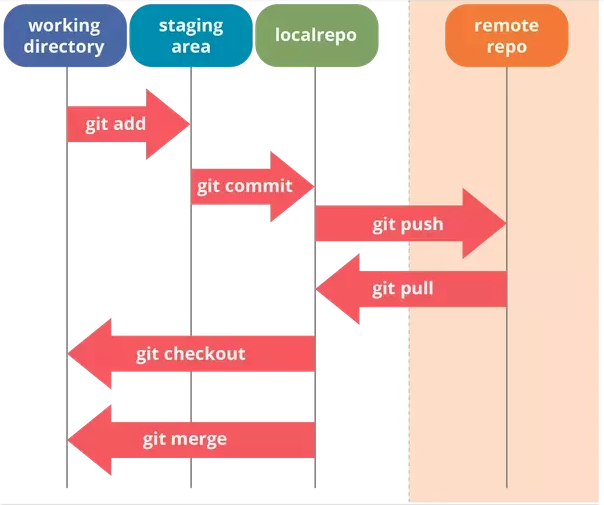
\includegraphics[width=1\textwidth]{github}
    \caption{Git und Github operationen}
    \label{fig:mesh1}
\end{figure}

\section{Projektboards}
Mit den Projektboards auf GitHub k\"onnen Softwareprojekte organisiert und Aspekte priorisiert werden. Projektboards k\"onnen f\"ur spezifische Funktionen, umfassende Roadmaps oder sogar Release-Checklisten erstellt werden. Projektboards bestehen aus Themen, Pull-Requests und Notizen, die in Spalten als Karten kategorisiert werden, zum Beispiel "To Do", "In Progress", "Ready to Review" und "Done". Notizen und Issues k\"onnen innerhalb einer Karte dargestellt werden und wechseln w\"ahrend ihrer Entwicklung die Karten / Spalten bis sie in der Karte "Done" bleiben. Dies kann sogar automatisiert werden. \cite{githubauto} $\newline$ 
Notizen und Issues k\"onnen Bugs, Features, Aufgabenerinnerungen oder Tasks welche in der Planungsphase anfallen, m\"ussen daher nicht direkt mit der Codebase zu tun haben. Neben Repository-weiten Projektboards gibt es auch Organisations-weite Projektboards, welche Probleme und Anfragen von allen Repositories beinhalten, die zu einer Organisation geh\"ort.

\section{Issues}
Viele Projekte sammeln Benutzerfeedback \"uber einen zentralen Bugtracker. GitHubs Tracker hei�t "Issues" und kann mit jedem Repository verwendet werden. Issues werden verwendet um Ideen, Erweiterungen, Aufgaben oder Fehler f\"ur die Arbeit an GitHub zu verfolgen. Issues k\"onnen von Usern und Entwicklern erstellt werden und k\"onnen zum Projektboard hinzugef\"ugt werden. Issues k\"onnen mehr als nur ein Ort zum Melden von Softwarefehlern sein. Ein Projektbetreuer kann mithilfe von Issues Tasks organisieren, die er ausf\"uhren m\"ochte, z. B. neue Funktionen hinzuf\"ugen oder alte \"uberwachen. Issues k\"onnen mit Pull-Requests verkn\"upft werden, damit sie bei der Ausf\"uhrung des Pull-Requests automatisch geschlossen werden. Issues k\"onnen auch anderen Benutzern zugewiesen, mit Labels (zum Beispiel "Bug", "Enhancement" oder "question") f\"ur eine schnellere Suche versehen und mit Meilensteinen gruppiert werden.

\pagebreak

\chapter{Anforderungen, Technologien}
\section{Anforderungsspezifikationen}
Die Software soll auf mobilen Ger\"aten sowie auf Desktop/Laptop Browsern benutzbar sein. Mobile Ger\"ate sind von der Leistung her meist schwach verglichen mit Desktopger\"aten. Server-side rendering kann dieses Problem weniger relevant machen, damit die Applikation nicht vollst\"andig vom Client berechnet werden muss. $\newline$
Die Website ist darauf ausgelegt, dass sie im Chrome Browser verwendet wird, da Chrome der verbreitetste Browser auf Android Ger\"aten ist, und auch seine Desktop Version sehr zuverl\"assig funktioniert. Apple ger\"ate k\"onnen ebenfalls Chrome verwenden. Chrome befindet sich auf den Meisten Ger\"aten auf dem neusten Stand und unterst\"utzt daher die meisten Funktionen. $\newline$
Als Testger\"ate werden ein Apple iPad und iPhone verwendet, ein Android Galaxy S5 und mehrere Macbook Pro und Air Laptops (ca. 2012 - 2016). $\newline$

\section{Progressive Webapp}
Um das Werkzeug "Waldmeister - Outdoors" nicht auf eine Plattform von Mobilen Ger\"aten zu beschr\"anken (iOS oder Android), setzt es auf die Prinzipien der Progressive Webapps (PWA). Diese beschreiben eine Website, die viele Merkmale besitzt, welche bisher den nativen Apps vorbehalten waren. Eine PWA ist gewissermassen eine responsive Website, welche auch offline verwendet werden kann. Sie schliesst dadurch eine zus\"atzliche Entwicklung einer nativen App, parallel zur Webseite \"uberfl\"ussig, da s\"amtliche Funktionen einer nativen App in der Webapp repliziert werden k\"onnen. Eine PWA erreicht diese offline F\"ahigkeiten durch den Einsatz von Service Workern; ein JavaScript, welches von Web-Browsern im Hintergrund ausgef\"uhrt wird. Einmal online aufgerufen, k\"onnen die Inhalte beim n\"achsten Besuch der Seite auch dann angezeigt werden, wenn eine schlechte oder sogar gar keine Internetverbindung besteht (Offline-Betrieb). Auch die von nativen Apps bekannten Push-Benachrichtigungen sind mit Service Workern m\"oglich. \cite{ServiceWorkers} $\newline$
Grundlegende Charakteristiken der PWA sind Offline Funktionalit\"at, Push Notifications, Add-To-Homescreen, jedoch ist keine Installation notwendig (beispielsweise \"uber den Apple Appstore oder Google Playstore). Verbreitete Mobile Browser wie Firefox und Google Chrome haben bereits eine vollst\"andige Unterst\"utzung von PWAs, Safari sollte dies bis Ende Februar 2018 ebenfalls implementiert haben und kann daher auch auf iOS verwendet werden. PWAs k\"onnen auf den Home-Screen des mobilen Ger\"ats hinzugef\"ugt werden.

\section{Mobile Field Solution mit ArcGIS Online}
Technologien von ESRI (Environmental Systems Research Institute) und insbesondere ArcGIS online wurden recherchiert, um einen funktionierenden Prototypen mit offline-caching zu erstellen. Hintergrundkarten (in Form eines Tile-Layers) k\"onnen auf dem Ger\"at zwischengespeichert werden. Die Erstellung von editierbaren Vektorlayern funktioniert auch beim offline Betrieb und k\"onnen sp\"ater, sobald wieder eine stabile Internetverbindung besteht, synchronisiert werden. Dieses Verhalten kann bei einer PWA durch Service-Worker rekreiert werden.$\newline$
Ein GeoJson file kann ebenfalls auf der online Plattform von ArcGIS hochgeladen werden und danach auf der Map dargestellt werden. Das Layer Styling kann so konfiguriert werden, dass die Farbe eines Polygons dem Typ des jeweiligen Waldstandorts entspricht.
 $\newline$

\begin{figure}[H]
    \centering
    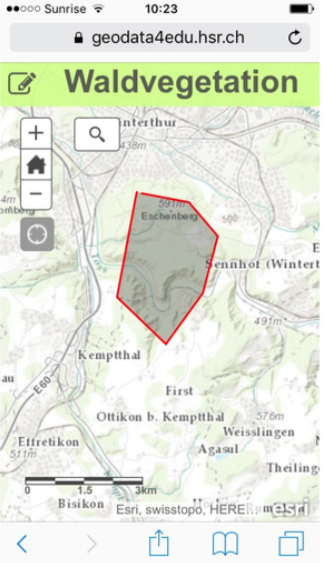
\includegraphics[width=0.5\textwidth]{esriprototyp}
    \caption{Prototyp mit ArcGIS online}
    \label{fig:mesh1}
\end{figure}


\section{Vue.JS}
Vue.JS ist ein JavaScript Framework, welches sich zum Erstellen von Single-Page-Webapplikationen in Form einer PWA eignet. Es wurde im Jahr 2013 erstmals ver\"offentlicht und wurde am 19. Dezember 2017 auf die aktuellste Version 2.5.13 gepatcht. Vue.JS folgt einer Variation des Model-View-Controller-Entwurfmusters, dem Model - View - ViewModel Muster. Wie auch das MVC folgt MVVM dient es der Trennung von Darstellung und der Logik der Benutzerschnittstelle. Dies erlaubt dem nutzenden Entwickler, die Struktur der Anwendung nach eigenen Anspr\"uchen zu richten. $\newline$
Entwickler beschreiben es daher als "less opinionated" im Vergleich zu anderen popul\"aren JavaScript Webframeworks wie Anglar.JS oder React. Vue.JS kann von Entwicklern eingesetzt werden welche HTML und JavaScript beherrschen und erfordert keine weiteren Webtechnologien. Vue.JS setzt eine Website aus Instanzen und Komponenten, bzw Single File Components zusammen. Single File Components sind bei VueJS, welche Architekturprobleme von mittel bis grossen Webapps, welche vollst\"andig von JavaScript getrieben werden, zu verbessern versucht. $\newline$
Folgende Probleme tauchen dabei auf:
$\newline$
\begin{enumerate}
\item Global definitions $\newline$
Global definitions force unique names for every component
\item String templates $\newline$
String templates lack syntax highlighting and require ugly slashes for multiline HTML
\item No CSS support $\newline$
No CSS support means that while HTML and JavaScript are modularized into components, CSS is conspicuously left out
\item No build step $\newline$
No build step restricts us to HTML and ES5 JavaScript, rather than preprocessors like Pug (formerly Jade) and Babel
\end{enumerate}
$\newline$
VueJS besagt, dass all diese Probleme von Single File Components (mit .vue extension) dank Werkzeugen wie Webpack und Browserify gel\"ost werden. Eine solche Komponente besteht auf HTML Template, JavaScript und CSS in einer eigenen, abgekapselten Datei. 
$\newline$
Durch das erzielt VueJS $\newline$

\begin{enumerate}
\item Complete syntax highlighting
\item CommonJS modules
\item und Component-scoped CSS
\end{enumerate}

Wem diese Idee Abkapselung nicht gef\"allt, der kann weiterhin ein CSS auslagern und in eine Komponente (innerhalb des HTML Templates) importieren: $\newline$
\begin{lstlisting}
<!-- my-component.vue -->
<template>
  <div>This will be pre-compiled</div>
</template>
<script src="./my-component.js"></script>
<style src="./my-component.css"></style>
\end{lstlisting}
$\newline$

\subsection{Separation of Concern}
Was ist gemeint mit Separation of Concern (SoC) und bricht der Aufbau von Single-File-Components nicht dieses Pattern? Eine bekannte Vorgehensweise bei Softwareengineering ist es, ein Computerprogramm in logische Abschnitte einzuteilen und zu separieren. Diese Teile sollten sich um einen Zweck oder Belang (Concern) k\"ummern. Dies heisst jedoch nicht, dass die verschiedenen Dateitypen unbedingt in separate Dateien aufgeteilt werden. In der modernen User Interface Entwicklung und den Entwicklern von VueJS ist es oft einfacher gefallen, verschiedene Komponenten, welche lose gekoppelt sind, zu komponieren, statt sie auf drei riesigen Layern (HTML, JS und CSS) getrennt zu halten, sie aber in den Komponenten zu verflechten. \cite{VueSFC} $\newline$
Auf diesem Weg sind Komponenten (Template, die Logik und das Styling) zusammenh\"angender und auch einfacher zu warten, obwohl dies nicht den Prinzipien von SoC folgt. Traditionelles SoC unterteilt dies in die Gruppen der Zwecke Organisation (HTML), Pr\"asentation (CSS) und Interaktion bzw. Verhalten (JavaScript)


\subsection{Vue-Router}
Der Vue-Router ist das Herzst\"uck einer Single-Page-Applikation (SPA). Der offizielle Vue-Router ist ein Client-seitiger Router, welcher mithilfe der HTML5 History API voll funktionsf\"ahiges Client-side routing macht. $\newline$ In der HTML Definition der Hauptkomponente kann <router-view> als Platzhalter verwendet werden, um die Komponenten anzuzeigen, welche abh\"angig von der momentanen Route an dieser Stelle angezeigt werden sollen. Ein Wechsel zwischen diesen Routen bewirkt kein Page-Reload, da dies von Vue.JS lediglich innerhalb derselben Page \"Anderungen bewirkt und keine tats\"achlichen URL Aufrufe ausf\"uhrt. $\newline$
Der Vue Router wird innerhalb einer Hauptseite angezeigt welche die Basis der Webseite darstellt. Methoden von Komponenten k\"onnen bewirken, dass sich der Inhalt ver\"andert, welcher an der Stelle des Router-Views angezeigt wird. Menupunkte im Header (z.B Register, Login, About, Map), bewirken mit .push() dass der Vue-Router mithilfe des index.js files die korrekten Komponenten an dieser Stelle anzeigt. Dies kann auch direkt \"uber eine URL Eingabe /register oder /login erfolgen, ohne dass der Aufruf \"uber eine interne Komponente ausgef\"uhrt werden muss. Die Datei index.js beinhaltet daher alle m\"oglichen Pfade, welche von der Webapp aufgel\"ost werden und bestimmt die angezeigten Komponenten, welche mit dieser Route verkn\"upft sind. $\newline$
Alternativ k\"onnten die \"ahnlichen L\"osungen von Page.js oder Director als Third-Party Produkte an dieser Stelle integriert  werden, es ist jedoch zu empfehlen, die offizielle Vue-Router Library zu verwenden.

\subsection{VueX}
VueX ist eine offizielle Erweiterung von Vue.JS und fungiert als Statusmanager. VueX arbeitet mit einem Store, welcher die Zust\"ande aller Komponenten in einer Vue Applikation \"uber Regeln definiert. VueX besteht aus Actions, Mutations und States. Aktionen k\"onnen in dieser Reihenfolge eine Auswirkung auf die Vue Komponenten haben. $\newline$
VueX hat Vorteile bei mittel bis grossen Projekten, welche auf dem Single-Page-Application Prinzip basieren. VueX bietet auch die M\"oglichkeit, einen zentralen Store in kleinere Module aufzuteilen, jedes mit ihren eigenen State, Mutations, Actions Werten. $\newline$
Da Komponenten in Vue abgekapselt sind, k\"onnen sie standardm\"assig nicht auf Daten zugreifen ,welche in anderen Komponenten definiert werden. Solche Daten m\"ussen per Store verf\"ugbar gemacht werden, damit sie \"uber mehrere Instanzen geteilt werden k\"onnen. $\newline$

\begin{lstlisting}
const sourceOfTruth = {}

const vmA = new Vue({
  data: sourceOfTruth
})

const vmB = new Vue({
  data: sourceOfTruth
})
\end{lstlisting}
$\newline$

Wird nun sourceOfTruth ver\"andert, wird sie in allen Komponenten, in welcher sie verwendet wird, automatisch auf den neuen Stand gebracht. Dies kann in gr\"osseren Applikationen schnell un\"ubersichtlich werden, da jede Komponente diese sourceOfTruth ver\"andern kann, ohne eine nachvollziehbare Spur zu hinterlassen. Es wird daher empfohlen, das Store Pattern von VueX zu implementieren, welche Ver\"anderungen am Store nur \"uber Mutationen zul\"asst. Somit wird es klarer, zu welcher Zeit welche Mutationen aufgerufen werden k\"onnen und wie sie durchgef\"uhrt wurden:$\newline$

\begin{lstlisting}
var store = {
  debug: true,
  state: {
    message: 'Hello!'
  },
  setMessageAction (newValue) {
    if (this.debug) console.log('setMessageAction triggered with', newValue)
    this.state.message = newValue
  },
  clearMessageAction () {
    if (this.debug) console.log('clearMessageAction triggered')
    this.state.message = ''
  }
}
\end{lstlisting}
$\newline$

\begin{figure}[H]
    \centering
    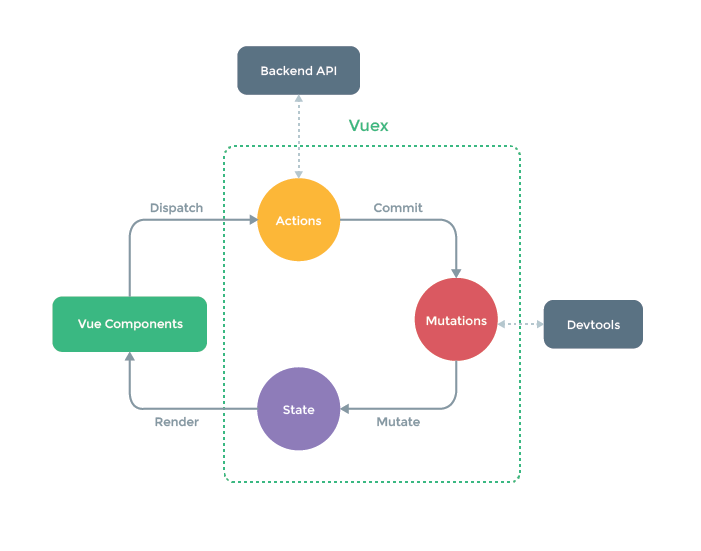
\includegraphics[width=1.25\textwidth]{vuex}
    \caption{Vuex Action-Mutations-State Diagram}
    \label{fig:mesh1}
\end{figure}

Komponenten k\"onnen auch private Zust\"ande haben, dies wird mit "privateState" erreicht. In diesem Fall muss der sharedState ebenfalls definiert werden.

\begin{figure}[H]
    \centering
    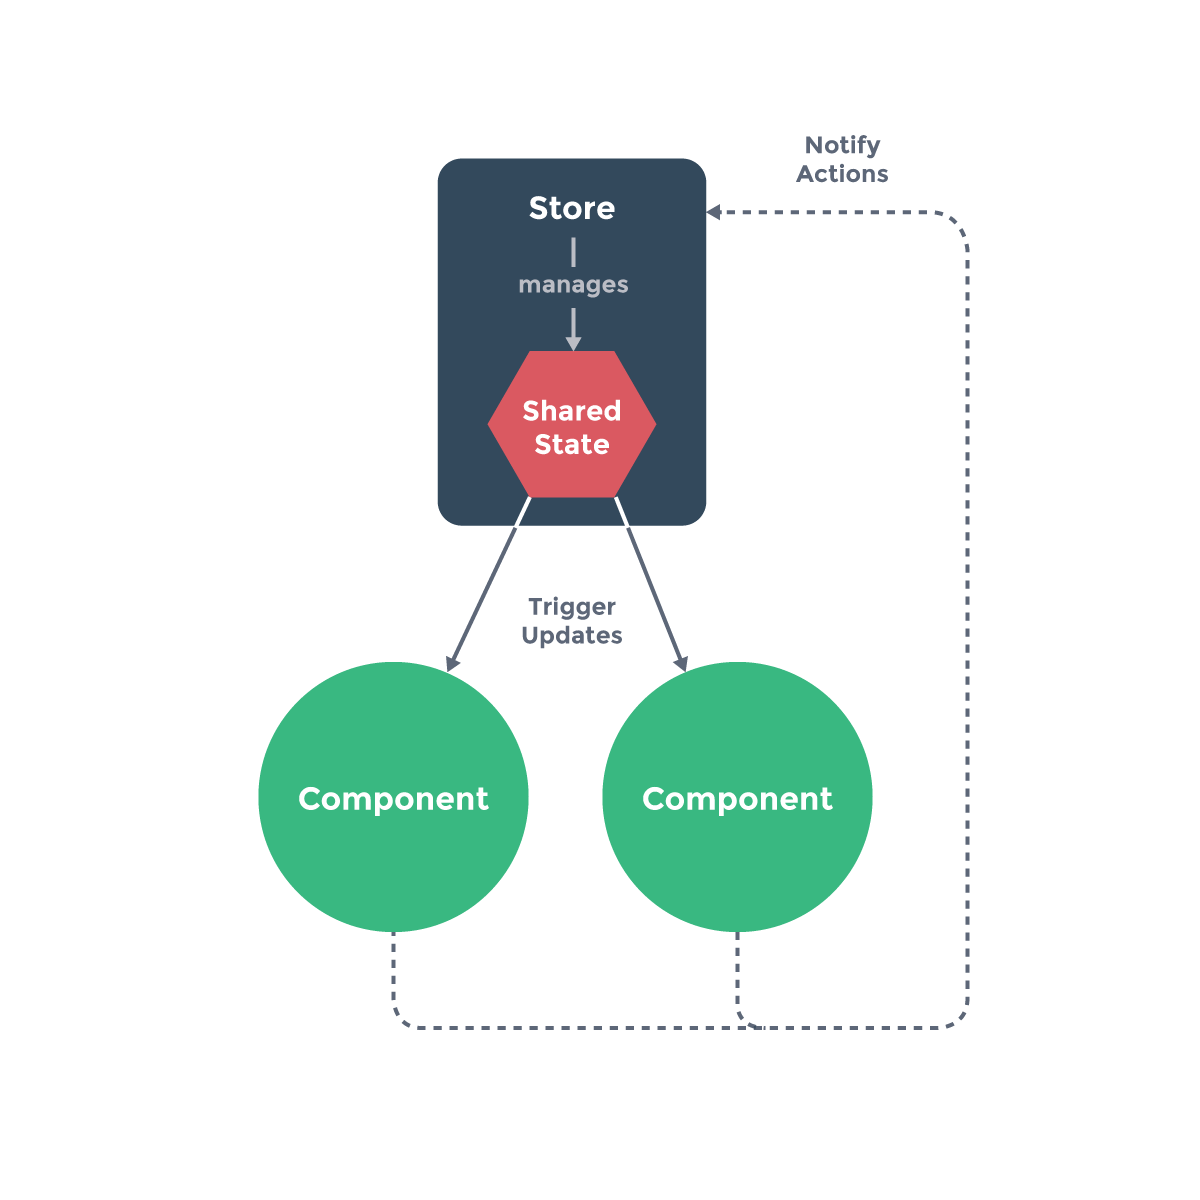
\includegraphics[width=1.25\textwidth]{sharedstate}
    \caption{Vuex private}
    \label{fig:mesh2}
\end{figure}

Dies bewirkt, dass eine Komponente nicht direkt einen Wert oder Zustand im Store ver\"andern kann, sondern dies einen Event aufruft. Dieser informiert den Store welchen State es \"uber eine Mutation zu ver\"andern gilt.


\subsection{Vuetify}
Vuetify ist eine Vue.JS UI Framework, welches das Frontend aus vielen Material-Design basierten UI Bausteinen zusammenbaut.

\section{Axios}
Axios ist eine JavaScript library zur Erstellung von Promise-Based HTTP Requests, welche "Waldmeister-Outdoors" dazu verwendet mit dem Server zu kommunizieren. Axios erm\"oglicht es, asynchrone HTTP requests zu REST Endpunkten abzusetzen oder Requests wie Create, Read, Update, Delete (CRUD) Operationen auszuf\"uhren. Axios kann in puren JavaScript Projekten verwendet werden oder auch in Projekten, welche auf Vue.JS basieren. Ein Promise-Objekt repr\"asentiert die in der Zukunft zu geschehende Komplettierung einer asynchronen Operation (oder deren Abbruch durch einen Fehler).

\section{Django}
Als Server zur Verwaltung der User und der Daten, welche die User generieren und ben\"otigen, kommt Django zum Einsatz. Es ist ein Open-Source Webframework, welches das Python Gegenst\"uck zu Ruby-On-Rails darstellt. Im Kern folgt es dem Model-View-Controller Prinzip, obwohl es eine eigene Namensgebung Verwendet. In diesem Projekt verwendet Django eine PostgreSQL Datenbank um Daten persistent zu machen. Django wird ebenfalls dazu verwendet um User einen Account zu geben, damit nur sie selbst Zugriff auf Ihre privaten Benutzerfl\"achen haben, oder um \"offentlich erstellte Benutzerfl\"achen mit anderen zu teilen.

\subsection{Django Rest Framework}
Eine SPA kommuniziert haupts\"achlich \"uber API Schnittstellen mit dem Server. Hier kommt auf dem Server das Django Rest-Framework (DRF) zum Einsatz. $\newline$
Es bietet ein sehr flexibles System zur Erstellung von RESTful Web-APIs. Das DRF bietet die M\"oglichkeit CRUD Operationen auf eine Ressource auszuf\"uhren. "Waldmeister-Outdoors" verwendet die REST Api beispielsweise um usergenerierte Fl\"achen, Pfade oder Punkte in der Datenbank zu speichern oder diese zur Darstellung in der Map aus der Datenbank zu laden. $\newline$
Ebenfalls werden Benutzer welche sich registrieren, mit Username, Password und ggf. Emailadresse in der Datenbank eingetragen. $\newline$

\section{PostgreSQL}
Postgres ist das Datenbank Management System, welches mit Django zusammen die Daten persistent macht, welche die User per API in der PWA generieren. Hierzu wird das Django Packet Psycopg2 verwendet. Django kann durch Models ein Datenbankschema beschreiben, welches von PostgreSQL generiert und in einer lokalen PostgreSQL Instanz gespeichert wird.

\subsection{PostGIS}
Um Geoinformationsdaten wie z.B. Polygone und Pfade korrekt zu speichern wird auf der Datenbank das Plugin PostGIS installiert. Dadurch kann Django die ben\"otigten Datenbankmodelle erstellen und per REST Schnittstelle speichern. Anhand des Django Models werden Geodaten in einem gew\"ahlten Format gespeichert. Standardm\"assig wird von Django die SRID 4326 (World Geodetic System, WGS84) verwendet. Dieses System benutzt Zahlen von -180, -90 bis 180, 90 um Positionen auf der Erde (in Latitude und Longitude) zu beschreiben. $\newline$
Postgis wird ebenfalls dazu verwendet, dass die Daten, welche per REST-Schnittstelle an den Client geschickt werden, in richtigem Format (Multipolygone in GeoJSON) \"ubermittelt werden.


\section{Leaflet}
Leaflet ist eine JavaScript Library, welche es erm\"oglicht, eine Map auf dem Client darzustellen. Es fokussiert sich auf Simplizit\"at, Performanz und ist sehr schlank, was einer PWA sehr entgegen kommt. Die Library ist nur 38 KB gross und erm\"oglicht es, viele Features zu verwenden, welche bei der Darstellung einer Map ben\"otigt werden, zum Beispiel Marker, GeoJSON Layer oder Buttons welche das Verhalten der Map beinflussen.

\subsection{TileLayer, Hintergrundkarte}
Der TileLayer fungiert als Hintergrundkarte, welche dynamisch geladen wird. Je nach ben\"otigtem Kartenausschnitt werden die Tiles als .pngs geladen und auf der Karte dargestellt. Dies f\"uhrt dazu, dass je nach Gr\"osse und Zoomstufe des Kartenausschnitts nur minimaler Datenaufwand bet\"atigt wird. Als Hintergrundkarte werden die "Terrain" Tiles von "stamen-tiles" verwendet.

\subsection{GeoJson Layer, Vegetationskundliche Karte}
Oberhalb der Hintergrundkarte wird ein GeoJson layer dargestellt, welcher die bereits bekannten Waldstandorte des Kantons darstellt. Er kann wahlweise ausgeblendet werden. Jedes Polygon dieses Layers wird durch ein Label beschriftet, welches den K\"urzel (EK72) dieses Waldstandorts beschreibt. Sie sind Ausdruck der Standorteigenschaften, und beziehen sich nicht auf die aktuelle
Bestockung, sondern auf eine potentielle nat\"urliche Vegetation. Die Farbe des Polygons wird ebenfalls \"uber diese Bezeichnung definiert und ist Teil des Standards Ellenberg Kl\"otzli (EK72).$\newline$
Diese Daten wurden vom Kanton Z\"urich bezogen und haben den Stand 31.12.1997. Viele Geometadaten haben jedoch den Stand 04. 04. 2011. $\newline$ Grundlage f\"ur die Digitalisierung bildeten masshaltige Folien aus der analogen Kartierung im Massstab 1:5'000. Der gr\"osste Teil wurde am damaligen Oberforstamt digitalisiert. Die Lagegenauigkeit ist c.a. 1 Meter. Die Daten wurden in der Form einer ESRI-Shapefile geliefert und mussten zuerst in das GeoJson Format transformiert werden, damit sie auf der Leaflet Map (als GeoJson Layer) dargestellt werden k\"onnen. Die Attribute (darunter die Kurzbezeichnung EK72) bleiben dabei erhalten. \cite{ZHGeoM}

\subsection{Leaflet editable}
Damit die User neue Polygone, Punkte und Pfade erfassen k\"onnen, ben\"otigt Leaflet das Plugin "Leaflet editable", welches es erm\"oglicht, neue Objekte direkt auf der Map zu zeichnen, oder bestehende Objekte zu editieren. Der User hat die M\"oglichkeit, dem Objekt per Dialogbox einen Namen als Label zuzuweisen, und zwischen den Zust\"anden privat oder public zu wechseln. Jeder User hat nur Zugriff auf seine eigenen privaten Fl\"achen, bzw. Pfade und Punkte, ausser er w\"ahlt es diese zu ver\"offentlichen, bzw "public" zu machen, damit sie alle User auf der Map sehen. Private Benutzerfl\"achen beschreiben oft Orte, welche w\"ahrend der Feldarbeit von pers\"onlichem Nutzen sind, jedoch f\"ur andere Experten nicht von Interesse sind oder bewusst privat gehalten werden. $\newline$
Sobald ein Objekt erfasst ist, wird es per REST Schnittstelle an den Server \"ubertragen und in der Datenbank gespeichert. 

\subsection{HTTPS, Geolocation}
Damit der eigene Standort auf der Map eingetragen oder die Map auf diesen Punkt zentriert werden kann, muss die Webapp HTTPS Secure (Https) verwenden, da die meisten Webbrowser es nicht zulassen, den Standort eines Users zu ermitteln, ohne dass die Verbindung gesch\"utzt ist. Um den Transport Layer zu verschl\"usseln wird ein self-signed Zertifikat verwendet, welches auf dem Vue-Client hinterlegt wird. Es besteht aus einer cert.pem und einer key.pem file. Browser werden zwar eine Warnung f\"ur solche Zertifikate einblenden, k\"onnen aber eine verschl\"usselte Verbindung aufbauen, nachdem sie zugelassen wird. $\newline$
Danach k\"onnen die Funktionen von HTML 5, z.B navigator.geolocation.getCurrentPosition() verwendet werden, welche einen Punkt mit Latitude und Longitude zur\"uckgibt. Zu diesem Punkt gibt es zus\"atzlich einen Accuracy Wert, welcher die Genauigkeit der Berechnung in Metern angibt.

\pagebreak

\chapter{Implementation}

\section{Mockup}
Die Mockups wurden vor der Implementation erstellt, um Screendesign und Layout klarer zu definieren, bevor es um die technische Implementation von "Waldmeister - Outdoors" ging. In den Abbildungen 1 bis 9 kann man den Arbeitsschritt Einloggen und Erstellen einer neuen Fl\"ache und eines Points of Interests (POI) sehen. Zus\"atzlich sieht der User seine eigene Location auf der Map eingetragen und hat \"uber das Menu "My Places" Zugriff auf eine Liste seiner erstellten Fl\"achen. Ein Kontextmenu gibt bei der Anzeige eines bestimmten Objekts zus\"atzliche Informationen.

\pagebreak

\begin{figure}[H]
\centering
    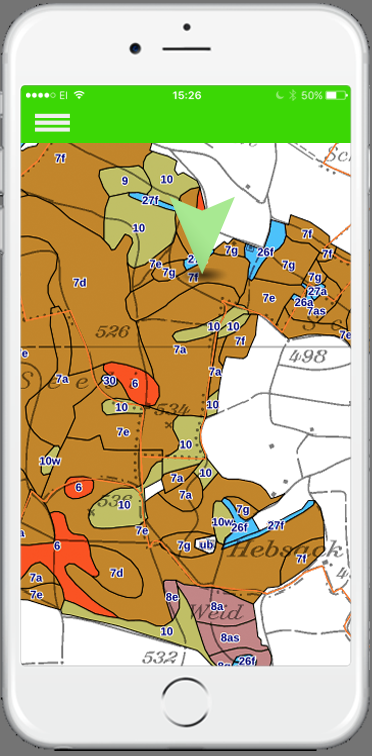
\includegraphics[width=0.7\textwidth]{mockup1-1}
    \caption{Mockup Screen 1}
    \label{fig:mesh1}
\end{figure}

\begin{figure}[H]
\centering
    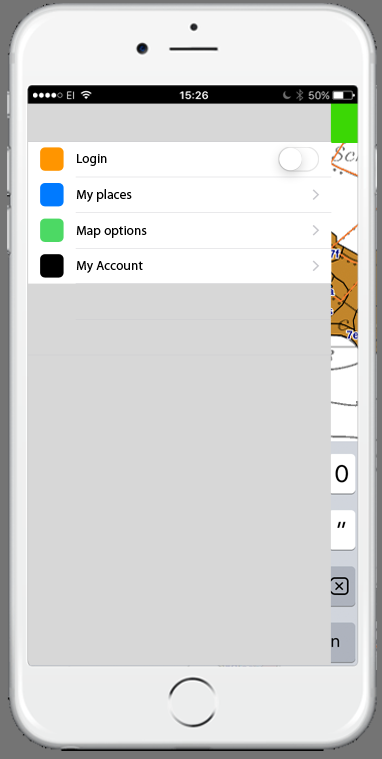
\includegraphics[width=0.7\textwidth]{mockup1-2}
    \caption{Mockup Screen 2}
    \label{fig:mesh2}
\end{figure}

\begin{figure}[H]
\centering
    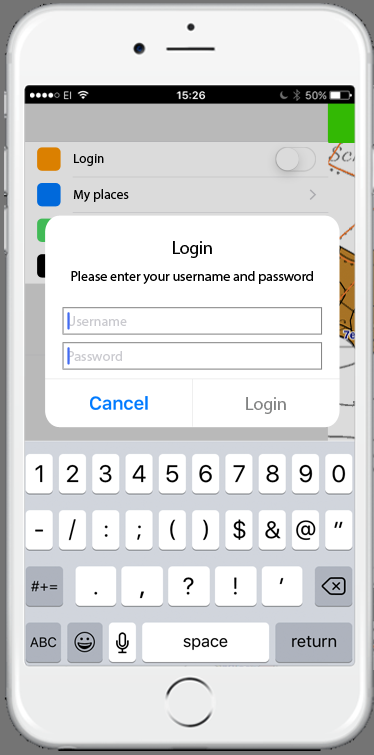
\includegraphics[width=0.7\textwidth]{mockup1-3}
    \caption{Mockup Screen 3}
    \label{fig:mesh3}
\end{figure}

\begin{figure}[H]
\centering
    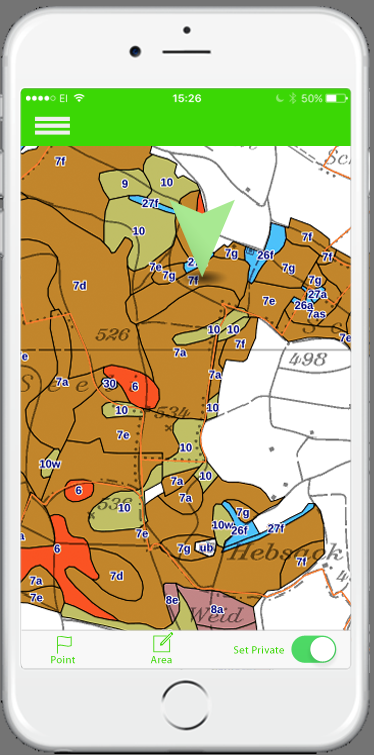
\includegraphics[width=0.7\textwidth]{mockup1-4}
    \caption{Mockup Screen 4}
    \label{fig:mesh4}
\end{figure}

\begin{figure}[H]
\centering
    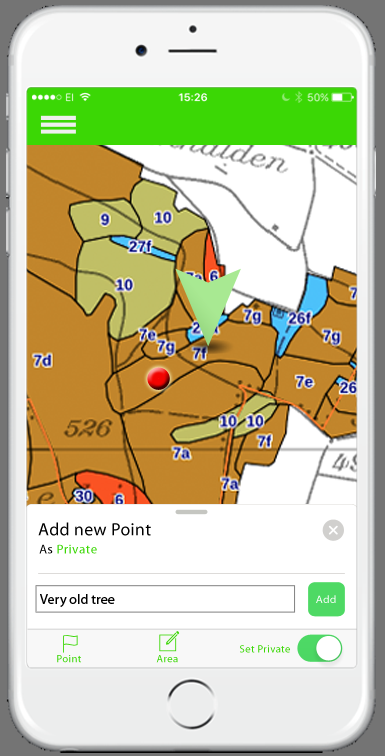
\includegraphics[width=0.7\textwidth]{mockup1-5}
    \caption{Mockup Screen 5}
    \label{fig:mesh5}
\end{figure}

\begin{figure}[H]
\centering
    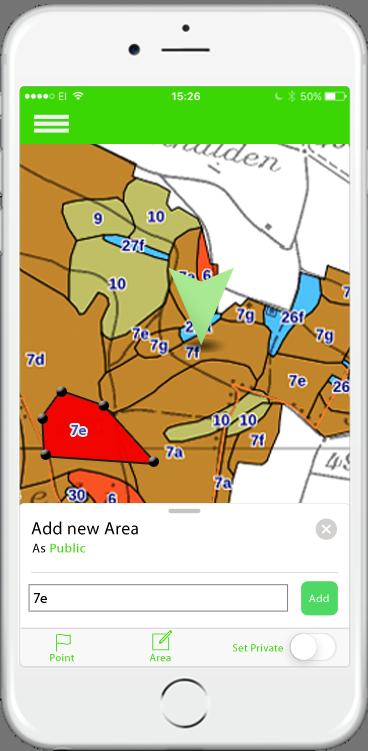
\includegraphics[width=0.7\textwidth]{mockup1-6}
    \caption{Mockup Screen 6}
    \label{fig:mesh6}
\end{figure}

\begin{figure}[H]
\centering
    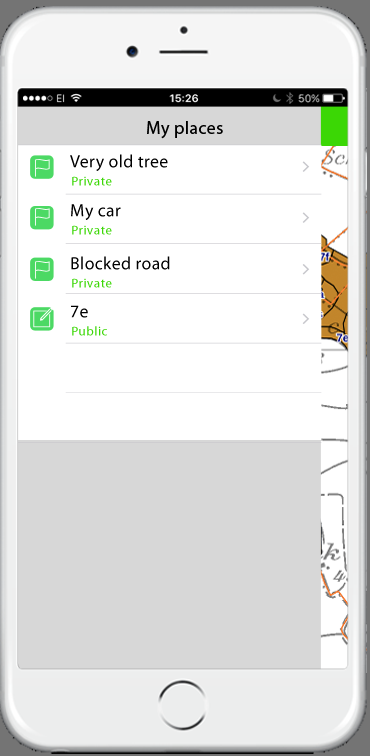
\includegraphics[width=0.7\textwidth]{mockup1-7}
    \caption{Mockup Screen 7}
    \label{fig:mesh7}
\end{figure}

\begin{figure}[H]
\centering
    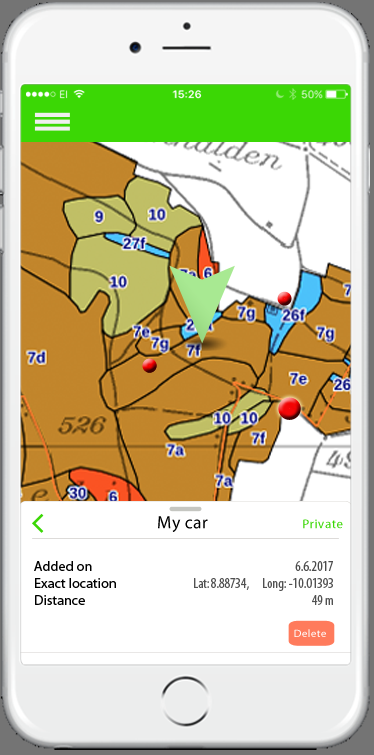
\includegraphics[width=0.7\textwidth]{mockup1-8}
    \caption{Mockup Screen 8}
    \label{fig:mesh8}
\end{figure}

\begin{figure}[H]
\centering
    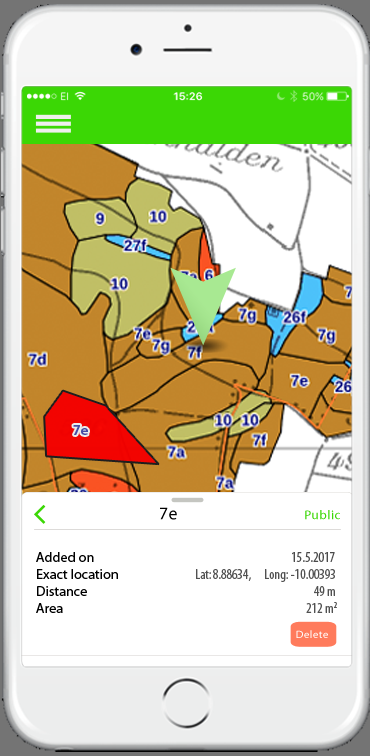
\includegraphics[width=0.7\textwidth]{mockup1-9}
    \caption{Mockup Screen 9}
    \label{fig:mesh9}
\end{figure}



\section{Modellierung mit UML Diagrammen}
UML Diagramme geben Auskunft \"uber die Architektur und Abl\"aufe des Systems. Es ist eine grafische Repr\"asentation in Form von Diagrammen, welche in der Sprache nach den Definitionen der "Unified Modeling Language" produziert sind. Diese bestimmt bei der Modellierung Beziehungen und Abh\"agigkeiten zwischen Begriffen und Notationen f\"ur diese Begriffe und statischen Strukturen und dynamischen Abl\"aufen. Modellierung und UML finden Verwendung und UML ist die dominierende Sprache f\"ur die Softwaresystem-Modellierung. Sie dient zur Kommunikation von Ideen zwischen Projektauftraggeber, Softwareentwickler und Systemingenieuren. $\newline$
In den 90er Jahren wurde die erste Spezifikation unter dem Namen UML 1.x entwickelt, im Jahr 2000 revidiert und in UML2 umbenannt. Seit Februar 2008 liegt Version 2.2 in der finalen Version vor. Seit Juni 2015 wird die aktuellste Version 2.5 verwendet. $\newline$
Haupts\"achlich definiert die Sprache Aktionen, Aktivit\"aten, Allgemeines Verhalten, Anwendungsf\"alle, Informationsfl\"usse, Interaktionen, Klassen, Komponenten, Kompositionsstrukturen, Modelle, Profile, Schablonen, Verteilungen und Zustandsautomaten. Diese kommen bei Strukturdiagrammen und Verhaltensdiagrammen zum Einsatz, wie u.a. den Klassen und Komponentendiagramm, oder Aktivit\"atsdiagramm, Sequenzdiagramm, Kommunikationsdiagramm, etc... Die Grenzen zwischen den \"uber vierzehn Diagrammtypen verlaufen weniger scharf. UML2 verbietet nicht, dass ein Diagramm grafische Elemente enth\"alt, die eigentlich zu unterschiedlichen Diagrammtypen geh\"oren. Elemente aus einem Strukturdiagramm und aus einem Verhaltensdiagramm k\"onnen nach Anwendungsfall auf dem gleichen Diagramm dargestellt werden, falls damit eine besonders treffende Aussage zu einem Modell gemacht werden kann. $\newline$


\subsection{Use Case - Diagramm}
Das Diagram \ref{fig:uc1} zeigt auf, welche M\"oglichkeiten ein User hat, mit dem Werkzeug zu interagieren. Ein User, welcher sich nicht registriert, kann keine Fl\"achen generieren oder editieren und kann auch keine privaten Fl\"achen sehen. Er kann jedoch die Vegetationskundliche Karte und \"offentliche Fl\"achen aller anderen User sehen. Nachdem er sich registriert und eingeloggt hat, kann er Fl\"achen erstellen und editieren. Diese teilen sich in \"offentliche und private Benutzerfl\"achen auf. Diese Option kann er w\"ahrend der Erfassung der Geometrie der Fl\"ache frei w\"ahlen. Standardm\"assig ist eine solche Fl\"ache privat und wird nur auf Wunsch des Users \"offentlich gemacht. Eine bereits erstellte Fl\"ache kann aber im Nachhinein auf \"offentlich umgeschaltet werden, nachdem sie z.B. durch \"Anderungen der Geometrie und Position vom User finalisiert wurde. Dies ist vorallem nach Absprache zwischen anderen Experten denkbar, welche \"uber Gruppen auch auf private, noch nicht \"offentliche Benutzerfl\"achen Zugriff haben um die Eigenschaften und Lage einer Fl\"ache zu analysieren und \"uber diese zu diskutieren.
\begin{figure}[h]
\centering
    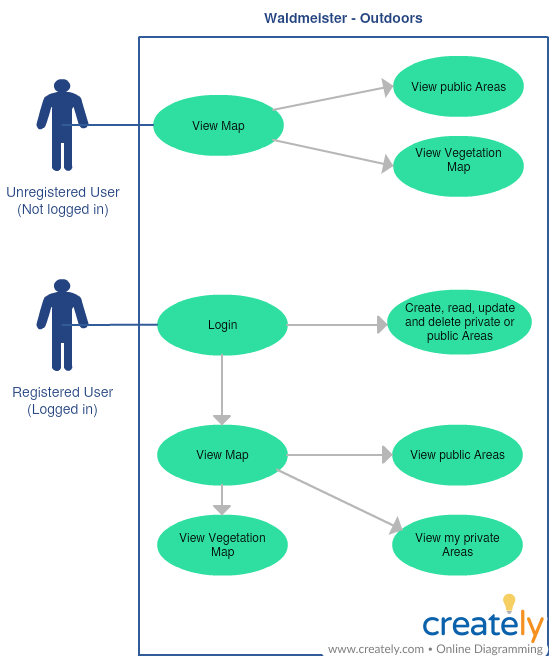
\includegraphics[width=0.9\textwidth]{WaldmeisterMap_USECASE}
    \caption{Use Case Diagram}
    \label{fig:uc1}
\end{figure}

\subsection{Klassendiagramm, Datenbankdiagramm}
Das Diagramm \ref{fig:cd1}  schildert die Relation und den Ausbau der wichtigsten Klassen des Systems. Dies zeigt, dass Benutzerfl\"achen nur von registrierten Users erstellt werden k\"onnen und immer einem solchen zugewiesen sind. Wird ein Benutzer aus dem System gel\"oscht, werden alle Fl\"achen welche diesem Account zugeordnet sind , ebenfalls aus dem System gel\"oscht. 

\begin{figure}[h]
\centering
    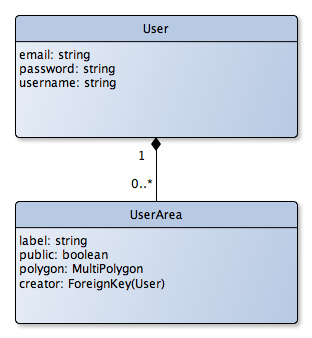
\includegraphics[width=0.5\textwidth]{ClassDiagram2}
    \caption{Klassendiagramm}
    \label{fig:cd1}
\end{figure}

\subsection{Sequenzdiagramm}

Die folgenden Sequenzdiagramme geben detaillierten Einblick in den Ablauf des Registrierung - und Loginvorgangs, sowie das Laden der Public und Private Areas und deren Darstellung im Client. $\newline$

\begin{figure}[H]
\centering
    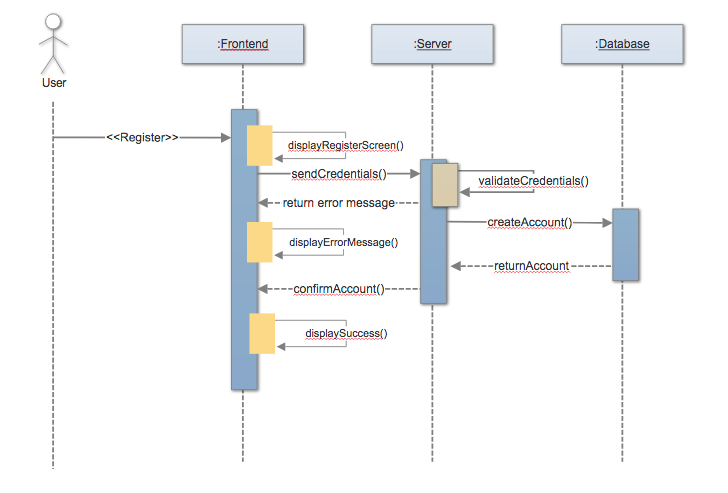
\includegraphics[width=0.9\textwidth]{Sequenz_DiagrammRegister}
    \caption{Sequenzdiagramm, Register}
    \label{fig:sd1}
\end{figure}

\begin{figure}[H]
\centering
    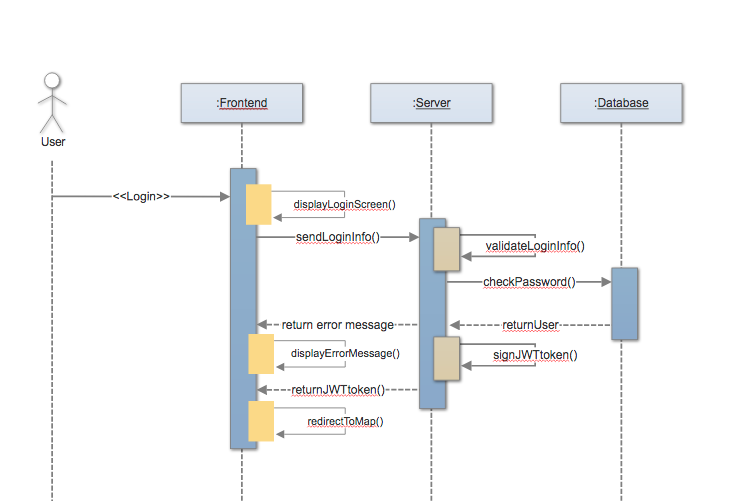
\includegraphics[width=0.9\textwidth]{Sequenz_DiagrammLogin}
    \caption{Sequenzdiagramm, Login}
    \label{fig:sd2}
\end{figure}

\begin{figure}[H]
\centering
    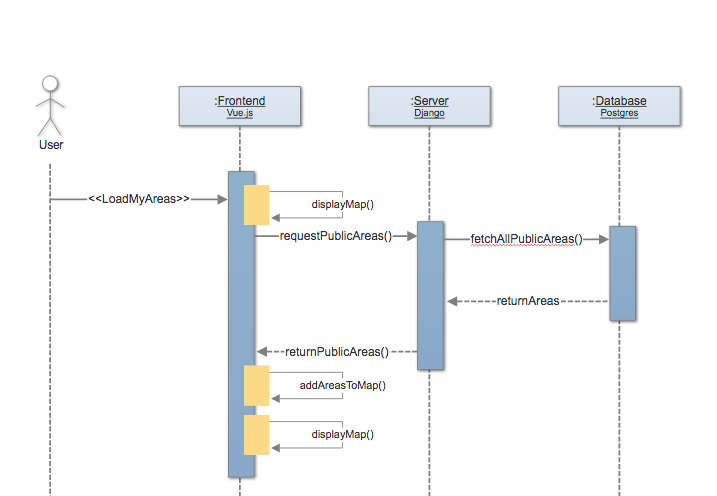
\includegraphics[width=0.9\textwidth]{Sequenz_DiagrammPublicAreas}
    \caption{Sequenzdiagramm, Public Areas}
    \label{fig:sd3}
\end{figure}

\begin{figure}[H]
\centering
    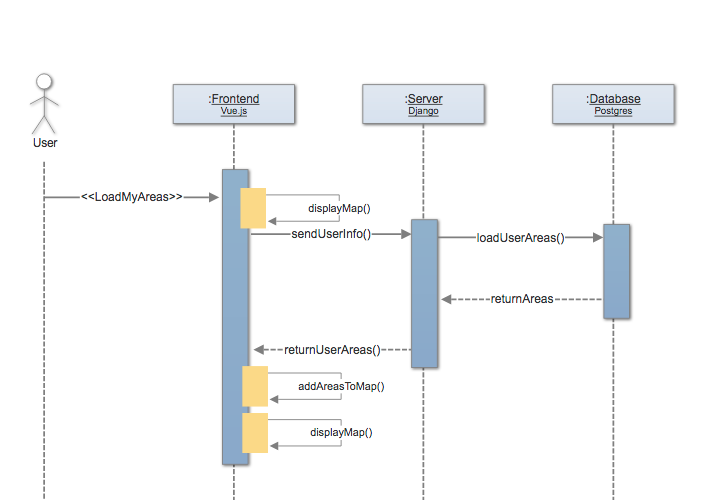
\includegraphics[width=0.9\textwidth]{Sequenz_DiagrammMyAreas}
    \caption{Sequenzdiagramm, My Areas}
    \label{fig:sd4}
\end{figure}

\subsection{Komponentendiagramm}

Das Komponentendiagramm zeit die Beziehungen zwischen verschiedenen Komponenten der Webapp. Die Waldmeistermap bezieht Daten \"uber verschiedene Interfaces welche auf der Map dargestellt oder verwendet werden.$\newline$

\begin{figure}[H]
\centering
    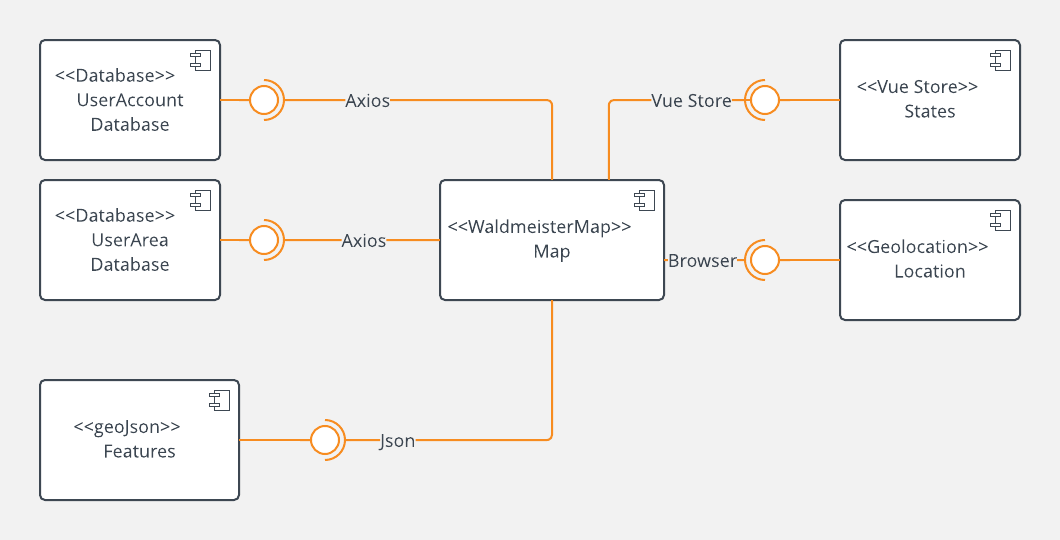
\includegraphics[width=1\textwidth]{umlwaldmeister}
    \caption{Komponentendiagramm, Waldmeister Map}
    \label{fig:kdwm}
\end{figure}

\pagebreak
\section{Technische Implementation}

\subsection{VueJS Komponenten}
Die Applikation "Waldmeister-Outdoors" setzt sich aus den Komponenten Register, Login, About, der WaldmeisterMap und einem Page Header zusammen. Dar\"uber hinaus bildet die Komponente "App.vue" die Basis, um den Page Header und Router-View Komponenten zu laden. $\newline$

\subsection{WaldmeisterMap}
Die Komponente WaldmeisterMap ist die Komponente, auf welcher die Leaflet Map und darauf die Layer Vegetationskarte (als geoJson) und der Layer f\"ur die Benutzerfl\"achen (als Polygone) dargestellt werden. Das leaflet Map Objekt beinhaltet auch die Kontrollbuttons, welche mit der Map assoziiert sind. Durch die Buttons 'Veg' und 'Areas' in der oberen linken Ecke der Map k\"onnen die GeoJson bzw die Benutzerfl\"achen ein - und ausgeschaltet werden. Dadurch werden die Layer, auf welchen sich die Polygone befinden gecleart und alle erstellten Labels von der Map gel\"oscht. Bet\"atigt der User den Button noch einmal, werden sie erneut erstellt. Sie sind standardm\"assig eingeschaltet und werden daher auch erstellt, wenn das Map Objekt auf die Page gemountet wird (beim Laden der WaldmeisterMap Komponente). Damit Label und Polygone der verschiedenen Layer separat ein und ausgeschaltet werden k\"onnen, werden sie zuerst in Gruppen unterteilt, bevor diese Gruppen auf die Map hinzugef\"ugt werden.$\newline$
Oberhalb dieser zwei Buttons befindet sich der "Add" Button, welcher es dem User erm\"oglicht, eine neue Benutzerfl\"ache auf der Map einzutragen. Er kann, w\"ahrend er im Zeichnungsmodus ist, per click event dem Polygon einen neuen Eckpunkt anh\"angen. Klickt der User w\"ahrend des Zeichnungsmodus auf den ersten erstellten Eckpunkt, schliesst sich das Polygon und der User wird per Dialogbox aufgefordert, dem erstellten Objekt die ben\"otigten Attribute zuzuweisen (label, public). Dr\"uckt er in diesem Dialog auf "Save" wird die Fl\"ache an den Server geschickt und in der Datenbank gespeichert. $\newline$

\subsection{Login und Registrierung}
Registrierung und Login werden als separate Komponenten aufgebaut, damit sie vom Vue-Router dargestellt werden k\"onnen. Sie beinhalten die Felder Username, Passwort und bei der Registrierung auch ein Email Feld, welches optional ist. Bei der erfolgreichen Registrierung wird von Djoser ein Benutzer angelegt und sein Passwort im verschl\"usselten Zustand hinterlegt. Loggt sich der Benutzer mit den korrekten Daten ein, erh\"alt er vom Server ein JWT (JSON Web Token), welches von Djoser basierend auf dem hinterlegten Accounts erstellt wird. Der Vue-Client Server hinterlegt dies in einem Store, damit es in verschiedenen Komponenten verwendet werden kann. Um sich dem Server gegen\"uber zu authentifizieren wird es bei einem Request mitgeschickt. Loggt er sich aus, wird dieses aus dem Store gel\"oscht. Der User kann sich erneut oder unter einem anderen Benutzernamen und Passwort einloggen. $\newline$
Bei nicht erfolgreichen Versuchen, einen Account zu erstellen oder sich einzuloggen, werden dem User diverse Fehlermeldungen angezeigt, welche Auskunft \"uber fehlerhafte Passworteingabe oder Benutzerdaten bei der Erstellung des Accounts geben. $\newline$
Nach einem erfolgreichen Login wird der User per Vue-Router auf die Komponente WaldmeisterMap weitergeleitet und alle Benutzerfl\"achen werden vom Server angefordert, auf die er Zugriff hat. Der Server liefert per REST Interface alle \"offentlichen Benutzerfl\"achen, sowie die privaten Benutzerfl\"achen, welche diesem User zugeordnet sind. \cite{djoserpack} $\newline$

\subsection{About}
Die Komponente About enth\"alt wichtige Informationen zu den dargestellten Daten und beinhaltet die Links zu den nativen iOS und Android Apps, unter welchen das Nachschlagewerk "Waldmeister" erh\"altlich ist. Unterhalb des dargestellten Logos befinden sich ausserdem Informationen zum Projekt und den Rahmenbedingungen, unter welchen es erstellt wurde. $\newline$
Hier wird auch dem Kanton Z\"urich gedankt f\"ur die Nutzungsrechte der Daten "Vegetationskundliche Kartierung der Waldfl\"achen im Kanton Z\"urich".

\begin{figure}[H]
\centering
    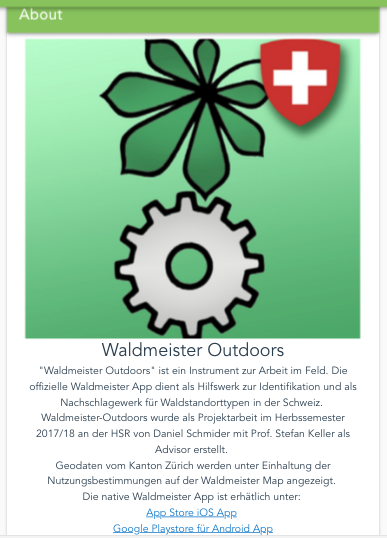
\includegraphics[width=0.5\textwidth]{aboutscreen}
    \caption{About in der Waldmeister-Outoors Webapp}
    \label{fig:aboutscreen}
\end{figure}

\subsection{User Interface / Frontend}
Das User Interface wurde gr\"osstenteils mit Vuetify realisiert, welches die \"aussere Erscheinung der Komponenten Header, Registrierung, Login, About, etc... bestimmt. Es wurde auf das Farbschema der existierenden Waldmeister App angepasst und eignet sich um eine Webapp responsive zu gestalten, damit sie auf mobilen Ger\"aten ebenfalls korrekt dargestellt wird. $\newline$
Weitere Teile, vor allem Elemente welche sich auf der Leaflet Map befinden, wurden mit CSS Styling aufgewertet. Der GeoJson Layer, welcher die Fl\"achen der Waldstandorte anzeigt, wird durch CSS dazu verwendet jedes Polygon auf diesem Layer aufgrund von einem Property des Polygons einzuf\"arben. Dieses Property ist die EK72 Kennzahl, bzw. K\"urzel. Jedem dieser K\"urzel kann eine bestimmte Farbe zugewiesen werden, welche als hexadezimale, 6-tellige Zahl im Code repr\"asentiert wird. Jedes Polygon erh\"alt dar\"uber hinaus auch ein Label, welches dieses K\"urzel ebenfalls darstellt. Diese Property Label haben eine weisse Schrift, sind nicht transparent und haben einen 2 Pixel weiten Schatten, damit sie sich von der Hintergrundfarbe abheben.$\newline$

\begin{figure}[h]
\centering
    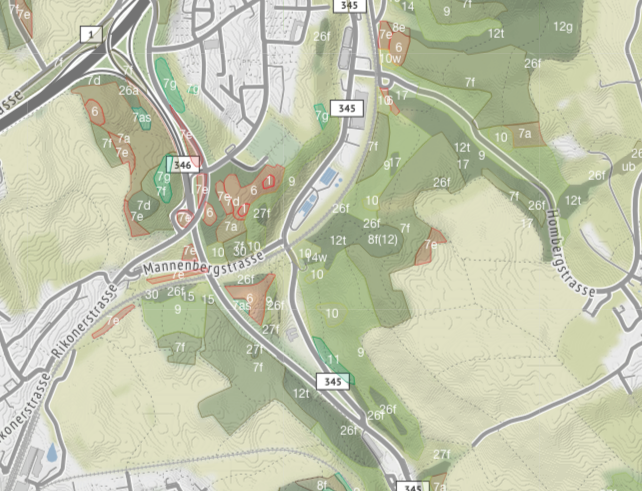
\includegraphics[width=1\textwidth]{propertylabel}
    \caption{Einf\"arbung von GeoJson Fl\"achen und Darstellung von PropertyLabels}
    \label{fig:propertylabel}
\end{figure}

$\newline$
Benutzerfl\"achen werden blau dargestellt und haben ein gef\"arbtes Label, damit sie sich von den Fl\"achen des geoJson Layers unterscheiden. Private Fl\"achen haben ein gelbes Label, \"offentliche sind gr\"un. Dar\"uber hinaus haben sie eine breitere Outline als Fl\"achen des GeoJson Layers.

\begin{figure}[H]
\centering
    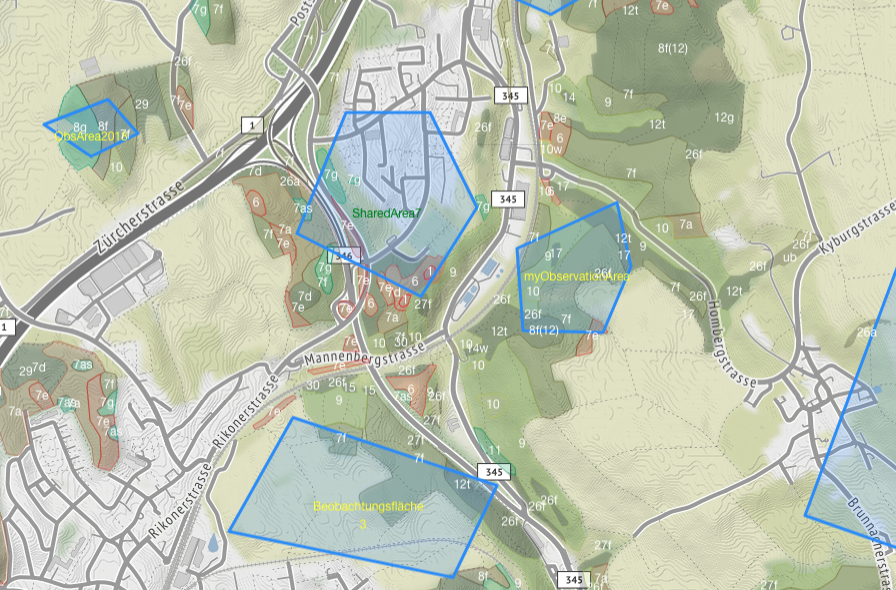
\includegraphics[width=1\textwidth]{userareas}
    \caption{Benutzerfl\"achen mit Labels}
    \label{fig:userareslabels}
\end{figure}

Die Geolocation wird als blauer "Circle" dargestellt. Die Gr\"osse des Kreises repr\"asentiert die Genauigkeit der Berechnung der Geolocation in Metern. $\newline$

\begin{figure}[H]
\centering
    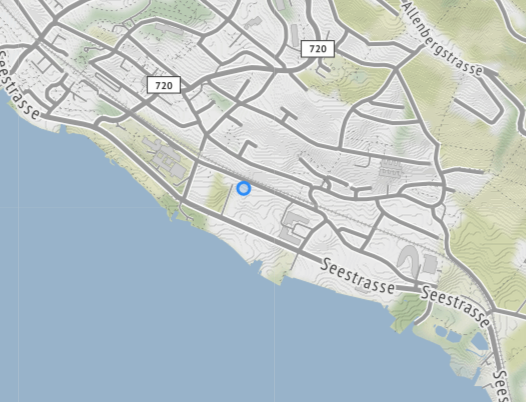
\includegraphics[width=1\textwidth]{geolocation}
    \caption{Geolocation mit Circle}
    \label{fig:geoloc1}
\end{figure}

Die Buttons welche den Zeichungsmodus starten oder beenden oder Ebenen ein- und ausblenden sind in der oberen linken Ecke, unterhalb der Zoombuttons vertikal aufgereiht. Der Zeichnungsbutton ist mit "Add" beschriftet und wechselt auf "Edit" solange der Zeichnugsbutton aktiviert ist. Die Buttons zum Ein- und Ausblenden von Ebenen sind mit "Veg" und "Areas" beschriftet, haben aber l\"angere Tooltips, welche die Funktion genauer beschreiben. $\newline$

Die "Save" Dialogbox wird nur angezeigt, wenn eine gezeichnete Fl\"ache durch einen Klick auf den ersten gezeichneten Eckpunkt geschlossen wird. Durch den "Save" Button innerhalb der Dialogbox werden die Werte f\"ur Label und Public \"ubernommen und das gezeichnete Polygon wird per REST Schnittstelle an den Server geschickt, damit es in der Datenbank gespeichert wird.
\pagebreak

\subsection{Axios Requests}
Diese Anfragen werden vom Client \"uber eine Axios API abgesetzt. Nach der Initialisierung des Axios Services wird eine Base Url bestimmt, welche auf das Backend im Django Server zielt. Mit jedem Request, welches \"uber diesen Service ausgef\"uhrt wird, wird auch das im Store hinterlegte JWT Token mitgeschickt, sofern es existiert. Falls nicht, wird der User als nicht autorisiert identifiziert.
Neben der Authentication Service, welcher die Methoden Register und Login ausl\"osen kann, besteht der AreaService, welcher per getAreas und postAreas Benutzerfl\"achen vom Server anfordern oder an den Server schicken kann, damit sie in der Datenbank erstellt werden. Die Erstellung von neuen Fl\"achen ist jedoch nur m\"oglich, wenn der User sich eingeloggt hat.$\newline$
Abh\"angig vom Request f\"ugt Axios Service eine URL-Endung an die Basisurl an, damit Django per Routingsystem erfassen kann um welche Art Request es sich handelt. Post Requests innerhalb des AuthenticationServices kommunizieren mit den Djoser definierten URL-Endungen /auth/users/create (um beispielsweise einen neuen Benutzer zu registieren). Diesem Post Request werden die credentials mitgeschickt, welche vom User im Client eingegeben wurden. Dieses credentials-Objekt besteht aus username, password und email. Sie werden als Json Objekt an den Django Server geschickt.$\newline$
Neben dem AuthenticationService regelt der AreaService per get und post requests \"uber die URL-Endungen '/api/areas/' Requests bez\"uglich Benutzerfl\"achen.
Axios kommuniziert mit dem Server \"uber eine REST-Schnittstelle. Benutzerfl\"achen werden per Get-Request an den Client \"ubertragen, neu erfasste Benutzerfl\"achen werden \"uber einen Post-Request als Json Objekte an den Server \"ubertragen. Django deserialisiert diese Json Objekte und speichert sie anschliessend in der PostgreSQL Datenbank. $\newline$

\subsection{Database Models}
Die Benutzerfl\"achen werden von Django durch ein Django-Dabatase-Model beschrieben und haben die Attribute "label, public, polygon und creator".  Label ist ein Feld welches aus Charakteren und Ziffern besteht. Die Maximall\"ange ist auf 50 Zeichen gesetzt, kann aber beliebig erh\"oht werden. $\newline$
Das Feld 'public' ist ein Boolean Wert, welcher bestimmt, ob eine Fl\"ache \"offentlich oder privat gehandhabt wird. $\newline$
'polygon' beinhaltet die Geometrie, die Art der Fl\"ache und das Format, in welcher sie in der Datenbank gespeichert wird. Die Geometrie ist Teil des polygon field und beinhaltet ein Array welches Punkte in Longitude / Latitude Paaren enth\"alt, die die Ecken des Polygons beschreiben. Dies k\"onnen beliebig viele sein und im Falle eines Multipolygons kann dieses Feld auch mehrere Arrays beinhalten, welche wiederum ein einzelnes Polygon beschreiben. \"Uberschneiden sich mehrere Polygone entstehen "Inseln", welche nicht zu der Fl\"ache des Multipolygons geh\"oren.$\newline$
Also Koordinatensystem wird das System WGS84 mit der SRID 4326 verwendet. \site{srid}

\subsection{Database, PostgreSQL}
Nachdem die Datenbank Modelle von Django definiert wurden, m\"ussen sie \"uber einen migrate Befehl in die PostgreSQL Datenbank \"ubertragen werden, damit sie erstellt werden. F\"ur die Kommunikation zwischen Django und PostgreSQL wird das Python Package Psycopg2 verwendet. Dieses Package ist der verbreitetste PostgreSQL Datenbank Adaptor f\"ur die Python Programmiersprache. $\newline$
Als Datenbank wird PostgreSQL 10 verwendet. Die Datenbank Verbindungsdetails sind in der Python settings.py Datei eingetragen. Waldmeister-Outdoors wird versuchen, auf eine lokale Datenbank mit dem Namen 'dschwaldmeister' zuzugreifen. Username ist postgres und der Port ist auf 5435 gesetzt, um Komplikationen mit anderen lokalen PostgreSQL Installationen zu vermeiden. Die "Engine" wurde ebenfalls auf 'django.contrib.gis.db.backends.postgis' ge\"andert, da postgis auf der Datenbank verwendet wird und als Extension installiert werden muss. Mit psql \"uber die Konsole oder PGAdmin4 k\"onnen auf die lokale PostgreSQL Datenbank zugegriffen, Daten manuell gel\"oscht oder eingetragen werden.

\subsection{API Dokumentation, Swagger}
Die API Dokumentation wurde mit dem Python Package Swagger implementiert und kann \"uber die URL WaldmeisterMap/swagger/ aufgerufen werden. Sie gibt Information \"uber alle verf\"ugbaren API Requests und deren Funktionen. Die API gliedert sich in die URLs der Benutzeraccount Erstellung (WaldmeisterMap/auth/) und die API Requests welche f\"ur die Erstellung von Benutzerfl\"achen zust\"andig sind (WaldmeisterMap/api/areas/). $\newline$
Benutzeraccounts werden vom Python Package Djoser erstellt. Dieses Package beinhaltet unter anderem die URL /WaldmeisterMap/auth/users/create/, welches mit den Attributen "email, username, password" einen neuen User in der Datenbank registriert. Nach der erfolgreichen Registrierung kann \"uber die URL /WaldmeisterMap/auth/token/create/ ein JWT Token vom Server angefordert werden. Dieser Request hat die Attribute "username, password". Stimmen die Werte mit einem existierenden Account in der Datenbank \"uberein, wird dem Client als Antwort ein JWT Token geliefert, welches der Client mit darauffolgenden Requests mitschicken kann, damit der Server den User mit einem registrierten User in der Datenbank verkn\"upfen kann. JWT Tokens laufen nach einer bestimmten Zeit ab oder z.B. wenn der Django Server sich neu initialisiert. Ein JWT Token kann \"uber die URL /WaldmeisterMap/auth/jwt/refresh/ erneuert werden, in dem das existierende Token im POST Request mitgeschickt wird.
$\newline$
Benutzerfl\"achen werden \"uber die URL /WaldmeisterMap/api/areas/ als GET Request abgefragt. Der Request liefert anhand vom eingeloggten oder nicht eingeloggten User \"offentliche Fl\"achen, bzw. auch die privaten Fl\"achen des authentifizierten Users, welche unter seinem Account in der Datenbank gespeichert sind. \"Uber die gleiche URL kann mit einem POST Request eine neue Benutzerfl\"ache in der Datenbank erstellt werden. \"Uber die URLs /WaldmeisterMap/api/areas/id kann auf eine spezifische, existierende Benutzerfl\"ache die Requests GET, DELETE, PATCH und PUT ausgef\"uhrt werden, um diese bestehende Benutzerfl\"ache zu bearbeiten, bzw. zu l\"oschen. Sie wird \"uber die URL-Endung "id" referenziert.

\begin{figure}[h]
\centering
    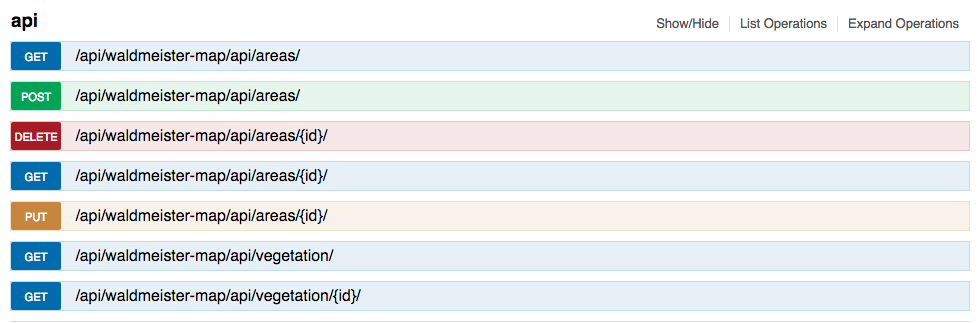
\includegraphics[width=1\textwidth]{swagger1}
    \caption{Swagger API Authorization}
    \label{fig:swagger1}
\end{figure}

\begin{figure}[h]
\centering
    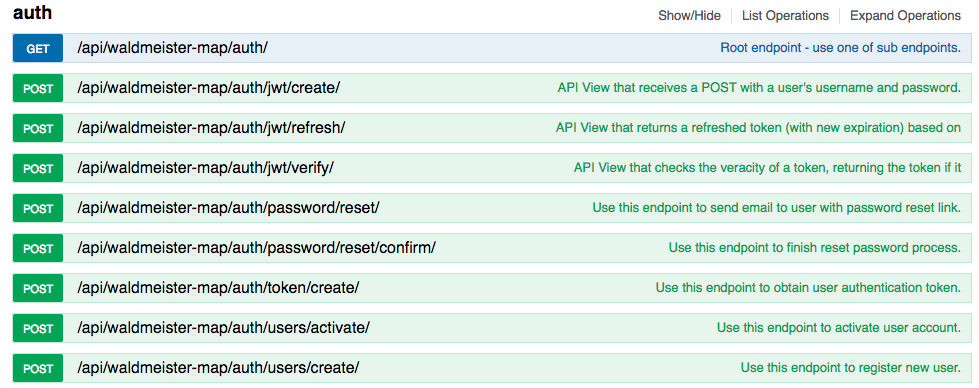
\includegraphics[width=1\textwidth]{swagger2}
    \caption{Swagger API UserAreas}
    \label{fig:swagger2}
\end{figure}

\begin{figure}[h]
\centering
    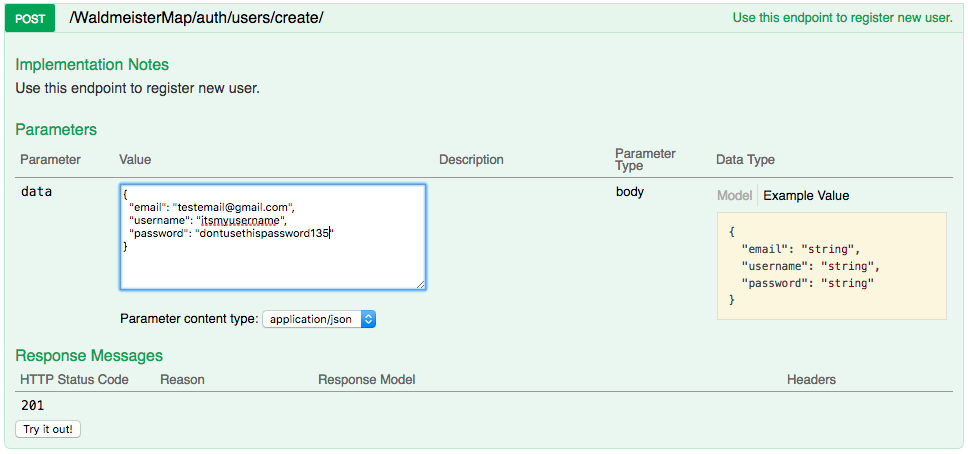
\includegraphics[width=1\textwidth]{swaggerdetails}
    \caption{Swagger API user create Details}
    \label{fig:swagger3}
\end{figure}

\clearpage
\pagebreak

\section{Tests}
\subsection{Unit Tests, TDD}
Testgetriebene Entwicklung (TDD) ist eine Methode zur Softwareentwicklung, welche oft bei der agilen Entwicklung von Computerprogrammen eingesetzt wird. Bei TDD erstellt der Programmierer Software-Tests, um das korrekte Verhalten von Softwarekomponenten zu planen und zu \"uberpr\"ufen. Unit Tests (auch als Unittest oder als Komponententest bezeichnet), werden verwendet um die funktionalen Einzelteile eines Softwareprojekts zu pr\"ufen. 

\subsection{VueJS}
Tests f\"ur Vue.JS wurden mit dem Test Runner Karma und dem Testframework Jasmine erstellt . Sie k\"onnen \"uber den Befehl "npm run test" ausgef\"uhrt werden, aus dem "client" folder des Vue-Servers. $\newline$
Getestet werden Komponenten und deren Inhalt, welche von VueJS verwendet werden. $\newline$
Damit Jasmin die tests ausf\"uhren kann, muss der Code von Webpack zuerst kompiliert werden. Danach wird er in einer Browserumgebung (z.B Chrome oder Firefox) ausgef\"uhrt und das Testframework sammelt die zu testenden Werte und Verhalten. Es vergleicht diese mit gegebenen Werten und Zust\"anden, welche vom Programmierer erwartet werden. Stimmen sie \"uberein, ist der Test bestanden. Stimmen sie nicht \"uberein, ist der Test gescheitert und Jasmine meldet einen Fehler.

\subsection{Django}
Test f\"ur das Django wurden mit dem standard Django module "unittest" erstellt. Es wurden Tests zu Login, Registrierung und Erstellung von Benutzerfl\"achen erstellt. Es werden unvollst\"andige, fehlerhafte und nicht authorisierte Requests (zum Beispiel ohne sich einzuloggen) getestet. HTTP-Statuscode geben Auskunft \"uber die korrekte Ausf\"uhrung oder fehlerhaftes Verhalten des Servers. Sie werden verglichen mit zu erwartenden Codes und bestimmen auf diese Weise ob der Test bestanden oder gescheitert ist. $\newline$

Es wird getestet ob Email und Passwort vorhanden ist und ob die Anforderungen an die Werte erf\"ullt sind, ob Accounts und JWTs erstellt werden k\"onnen und ob Benutzerfl\"achen vom System korrekt erstellt werden. $\newline$
Die Tests k\"onnen mit dem Befehl "python3 manage.py test WaldmeisterMap" ausgel\"ost werden. Fehlerhafte Test werden von Django gemeldet.

\pagebreak

\chapter{Resultate}
Das Projekt wurde mit genannten Technologien umgesetzt und wird auf Github gehostet: $\newline$
https://github.com/dschmide/Waldmeister
Installationsanleitung im Readme und im Kapitel Softwaredokumentation weiter unten in diesem Dokument.
$\newline$

\section{Erreichte Ziele}
User k\"onnen mittels der Webapp Waldmeister-Outdoors die Vegetationskundliche Karte erforschen und diese mit Ihrem momentanen Standort abgleichen. Dar\"uber hinaus k\"onnen sie, nachdem sie sich registriert haben, private und \"offentliche Benutzerfl\"achen auf einem mobilen Ger\"at erfassen und sie auf einem zentralen Server hinterlegen. Somit k\"onnen sie pers\"onliche Orte und Fl\"achen gebrauchen, welche f\"ur Sie im Arbeitsalltag relevant sind und sie zwischen verschiedenen Ger\"aten (Im Feld und im B\"uro) abrufen oder mit anderen Personen teilen, wenn sie die Fl\"ache \"offentlich und daher von allen Usern abrufbar machen. $\newline$
Ebenfalls wurde erreicht die Geolocation auf der Karte darzustellen. Dies ist im Arbeitsalltag eine grosse Hilfe, und dient zur schnellen Orientierung und Auffindung von bestimmten eingetragenen Fl\"achen und Orten im Feld. $\newline$
Die Webapp kann sowohl auf Desktop Browsern wie von mobilen Ger\"aten verwendet werden und verh\"alt sich dank Vue.js responsive auf eine \"Anderung des Viewports, zum Beispiel wenn der Screen eines mobilen Ger\"ats w\"ahrend der Verwendung gedreht wird. $\newline$
Layer und deren Label k\"onnen ein - und ausgeblendet werden, was zur \"Ubersicht beitragen kann. $\newline$
Alle Benutzeraccounts und deren Fl\"achen sind im Django Backend ersichtlich und k\"onnen als Superuser ver\"andert oder gel\"oscht werden. Wird ein Benutzer aus der Datenbank gel\"oscht, werden alle von ihm erstellten Benutzerfl\"achen ebenfalls automatisch gel\"oscht. Alle Passw\"orter von Benutzeraccounts werden gehasht in der Datenbank gespeichert. $\newline$


\section{Verbesserungen, Weiterentwicklungen}
\subsection{Automatische Standortbestimmung}
Die automatische Bestimmung, in welchem Waldstandort sich ein User anhand der Geolocation befindet, ist ein w\"unschenswertes Feature, da es den User laufend dar\"uber informiert, in was f\"ur einem Waldtyp er sich befindet, ohne dass er dies durch einen Aufruf selbst ausf\"uhren muss. Dies kann erreicht werden durch eine periodische Abfrage der Geolocation, gekoppelt mit einer Berechnung in welchem GeoJson Polygon sich dieser Punkt befindet. Eine solche Berechnung ist zum Beispiel \"uber die Library geojson-geometries-lookup m\"oglich, welche alle Polygone aus einem GeoJson zur\"uckgibt, welche den gegebenen Punkt beinhalten. Danach kann aus dem EK72 Feld der K\"urzel ausgelesen und dem Benutzer angezeigt werden. \cite{GeoLookup} $\newline$
Um diesen Ablauf f\"ur den User so angenehm wie m\"oglich auszuf\"uhren, k\"onnte er in der Toolbar in einen Tab wechseln, welcher keine Map, sondern lediglich die Information darstellt, in welcher Waldfl\"ache er sich befindet. Dies kann in einem gegebenen Intervall automatisch wiederholt werden. $\newline$

\subsection{Editieren und L\"oschen von erstellten Benutzerfl\"achen}
Ein weiteres geplantes Features ist es, die Geometrie oder das Label von erstellten Benutzerfl\"achen zu editieren, sie vom erstellten Zustand (\"offentlich oder privat) in einen anderen zu wechseln oder sie wieder zu l\"oschen, damit sie nicht mehr in der Datenbank eingetragen sind. Dies vervollst\"andigt die CRUD Operationen, welche in einer solchen Anwendung w\"unschenswert sind.$\newline$
Der Server, bzw. die REST-Schnittstelle l\"asst diese Operationen bereits zu (siehe API Dokumentation), sie sind jedoch im Frontend noch nicht eingebaut.

\subsection{Auflistung der Benutzerfl\"achen}
Um die Lokalisierung von bereits erstellten Benutzerfl\"achen zu erleichtern, w\"are es von Vorteil, diese in einer geordneten Liste darzustellen, z.B. in alphabetischer Reihenfolge oder nach ihrem Erstellungsdatum. Klickt der User auf eine dieser Listeneintr\"age, w\"urde die Map auf die Lage dieser Fl\"ache fokussieren. $\newline$
Eine solche Auflistung w\"are als aufklappbares Menu denkbar, welches sich \"uber einen Button im Header der Applikation auf - und zuklappen l\"asst.

\subsection{Gruppen}
User von Waldmeister-Outdoors sollen Gruppen erstellen k\"onnen und andere Benutzer einladen, um Fl\"achen unter sich zu teilen. Dies hat zum Vorteil, dass die Benutzerfl\"achen nicht \"offentlich abrufbar, aber innerhalb einer Gruppe sichtbar sind. Die Gruppe kann so \"uber mehrere Ger\"ate gleichzeitig \"uber eine Benutzerfl\"ache diskutieren oder sie auch bearbeiten, bevor sie ver\"offentlicht wird. $\newline$
Das Kreieren, Betreten oder Verlassen einer Gruppe sollte m\"oglichst einfach \"uber einen Punkt im Menu m\"oglich sein. Der User, welcher die Gruppe erstellt hat, sollte dabei Einladungen verschicken bzw. Gruppenmitglieder wieder aus der eigenen Gruppe l\"oschen k\"onnen. Denkbar ist auch, anderen Gruppenmitgliedern Rechte zu erteilen, andere User einzuladen.

\subsection{Pfade und Orte}
Neben Fl\"achen k\"onnen auch Pfade und Orte eine unterst\"utzende Funktion im Feld darstellen. Um Pfade zu erstellen k\"onnen beispielsweise vergangene geolocations des Users zu einem Pfad zusammengef\"ugt werden, welcher die zur\"uckgelegte Strecke darstellt. Mithilfe von Timestamps w\"are es m\"oglich, den Tagesablauf zu protokollieren und sie mit einer T\"atigkeit an einem Ort zu verkn\"upfen. $\newline$
Orte, sogenannte Points of Interests (PoI), k\"onnten Teammitglieder oder andere Experten auf bestimmte Indikatoren, wichtige \"ortliche Gegebenheiten hinweisen, den Standort des n\"achstgelegenen Parkplatzes oder eine unterbrochene Zufahrtsstrasse kennzeichnen. Diese Orte m\"ussen nicht durch eine Fl\"ache beschrieben werden, sondern nur durch einen einzigen zweidimensionalen Punkt. $\newline$
Zu Orten, bzw auch Fl\"achen k\"onnte ein Bild hochgeladen werden, um die Stelle genauer zu kennzeichnen, oder um mit anderen Experten \"uber den Standort zu diskutieren.

\subsection{Continuous Tracking}
Die Map wird nur in dem Zeitpunkt in dem sie geladen wird auf die momentane Geolocation des Users zentriert. Dieses Feature k\"onnte erweitern werden, indem der angezeigte Kartenausschnitt gewissermassen dem User folgt. Wiederholend in einem kurzen Intervall soll die map automatisch auf die Geolocation des Ger\"ats zentriert werden. Auf diese Weise wird der User stetig in der Mitte der Karte angezeigt. $\newline$
Dieses Feature kann jedoch je nach Anwendungsfall als st\"orend empfunden werden und sollte deaktivierbar sein, bzw. nur auf Aufforderung des Users aktiviert werden.

\subsection{Plus Codes}
Plus Codes k\"onnen verwendet werden, um Koordinaten in eine Zeichenfolge umzuwandeln. Es wird dazu verwendet, einem Ort auf der Welt gewissermassen eine Adresse zu geben, \"ahnlich wie eine Strassenadresse. Statt einen Punkt in geografische Breite und L\"ange zu beschreiben, ist die Zeichenfolge lediglich 7 oder 11 stellig (Eine Stelle ist dabei immer das namengebende + oder - Zeichen, welches die Zeichenkette auch von internationalen Postleitzahlen abhebt). Je nachdem, ob der Code einen Ort lokal oder weltweit beschreibt, k\"onnen die vier ersten Ziffern weggelassen werden, da es ersichtlich ist, um welche weltweite Region (ca. 100 Kilometern) es sich handelt. Dies funktioniert \"ahnlich wie eine Vorwahl bei Telefonnummern, welche regional nicht ben\"otigt wird. Die vollst\"andige Zeichenfolge beschreibt einen Ort auf dem Planeten mit einer Genauigkeit von 14 auf 14 Metern. Es kann jedoch ein weiteres Zeichen angeh\"angt werden, um die Genaugkeit auf drei auf drei Meter zu erh\"ohen. Plus Codes beschreiben immer eine Fl\"ache, keinen genauen Punkt.$\newline$
Plus Codes k\"onnen offline en- oder dekodiert werden.  \cite{PluCo} $\newline$
Sie basieren auf Open Location Code (OLC), ein open-source Projekt welches von Google in Z\"urich entwickelt wurde. Das Projekt ist auf Github gehostet unter https://github.com/google/open-location-code. Es existieren Libraries f\"ur JavaScript wie auch Python. $\newline$
"Waldmeister Outdoors" kann diese Codes gebrauchen, damit Experten unter sich einfacher Geolocations austauschen k\"onnen. Die Webapp kann jeder Fl\"ache einen solchen Code zuweisen, nachdem die Benutzerfl\"ache vom User erstellt wurde. Der Code repr\"asentiert das geometrische Zentrum der Benutzerfl\"ache, welches von Leaflet berechnet wird.

\pagebreak 

\section{Screenshots}

\begin{figure}[h]
\centering
    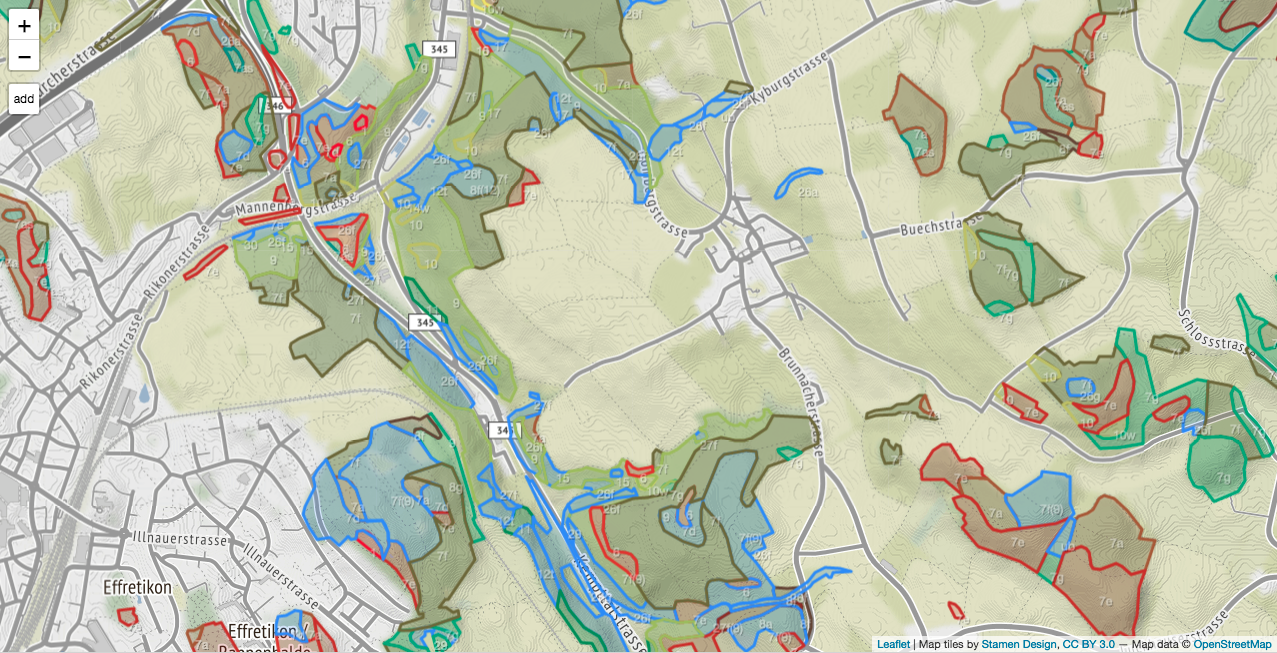
\includegraphics[width=1.1\textwidth]{ScreenShot}
    \caption{Screenshot Desktop, Vegetationskundliche Karte}
    \label{fig:ss1}
\end{figure}

\begin{figure}[h]
\centering
    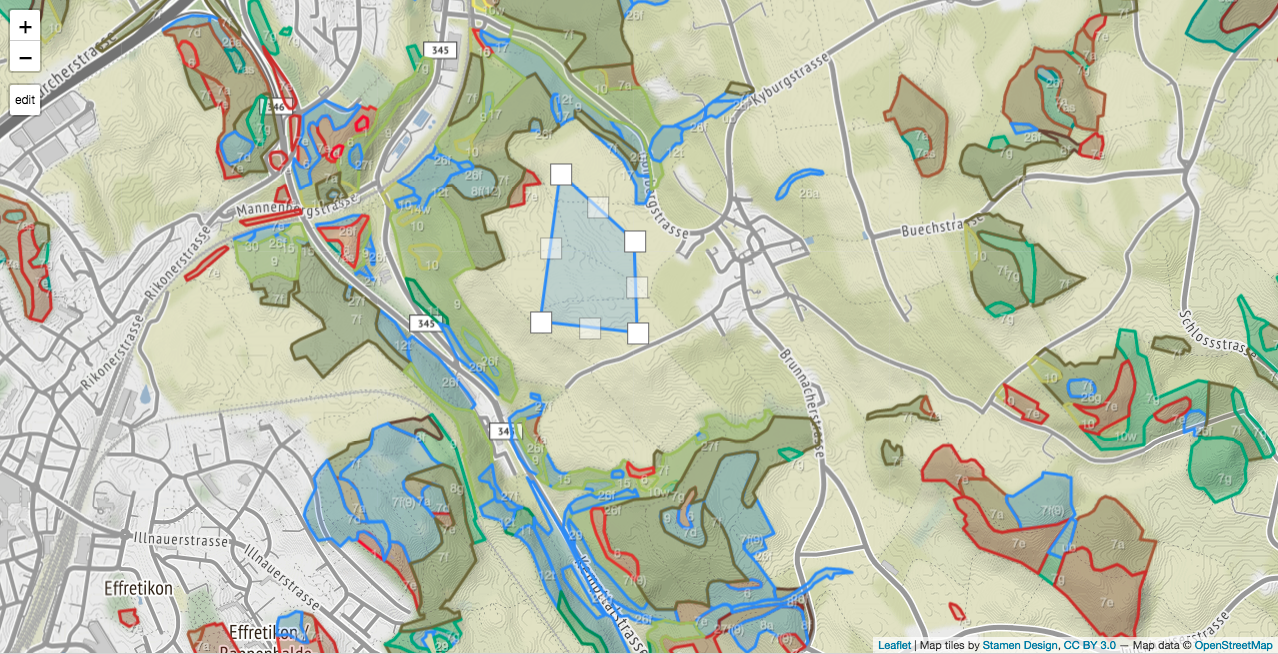
\includegraphics[width=1.1\textwidth]{ScreenShot2}
    \caption{Screenshot Desktop, EditArea}
    \label{fig:ss2}
\end{figure}

\begin{figure}[h]
\centering
    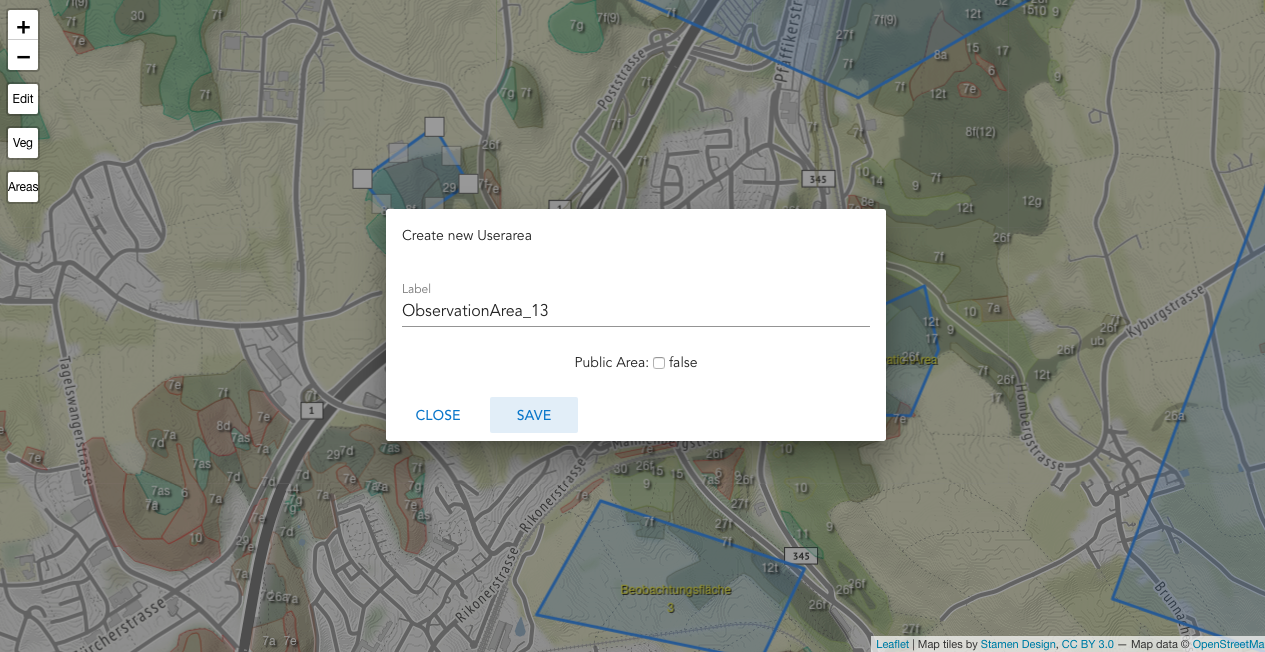
\includegraphics[width=1\textwidth]{overlay}
    \caption{Screenshot Desktop, Dialogbox}
    \label{fig:ss2}
\end{figure}

\pagebreak

\chapter{Softwaredokumentation}
\section{Installation}
Um die App zu verwenden, sollte die Anleitung auf GitHub (Readme) verwendet werden. $\newline$
$\newline$
Github Repo klonen $\newline$
"npm install" $\newline$
"npm start" im client folder startet den Vue-Server $\newline$
"python manage.py runserver" (als separates Window oder Tab) im root folder started den Django Server $\newline$
Damit Django die PostgreSQL Datenbank verwenden kann, m\"ussen die Werte in der settings.py angepasst werden, oder eine Datenbank mit dem Namen dschwaldmeister, user Postgres und Port 5435 erstellt werden. Von PostgreSQL soll auch die Extension postgis erzeugt werden. $\newline$
Mit "manage.py migrate" kann die Datenbank auf den neusten Stand gebracht werden, damit sie verwendet werden kann. $\newline$
Die App kann im Browser unter der angezeigten Adresse des Vue-Servers aufgerufen werden. $\newline$



\pagebreak

\chapter{Links}
\subsection{github und maps.zh}
Projekt Wiki $\newline$
https://wiki.hsr.ch/StefanKeller/wiki.cgi?PA2_Schmider_Aufgabenstellung $\newline$
https://giswiki.hsr.ch/Koordinatensystem $\newline$
Github und Github Projekt $\newline$
https://github.com/dschmide/Waldmeister $\newline$
https://github.com/dschmide/Waldmeister/projects/1 $\newline$
Gis-Browser Kanton Z\"urich $\newline$
https://maps.zh.ch?topic=WaldVKZH&scale=18634&x=2706590.13&y=1251180.39&srid=2056 $\newline$
Native Apps f\"ur Android und iOS Ger\"ate $\newline$
https://itunes.apple.com/bn/app/waldmeister/id825753160?mt=8 $\newline$
https://play.google.com/store/apps/details?id=bgu_schmider.waldmeister $\newline






